\section{Additional uncertainty scans}
\label{sec:appendix_performance}

The seven one-dimensional scans not shown in Sec.~\ref{sec:uncertainties}, in the
same format: the predicted \ggHH cross section along one Wilson coefficient
with the other eight at zero, the interpolation uncertainty of
Eq.~\eqref{eq:sigmainterp}, and the same uncertainty as a fraction of the yield
in the lower panel. The dotted line is the SM.

\begin{figure}[htbp]
    \centering
    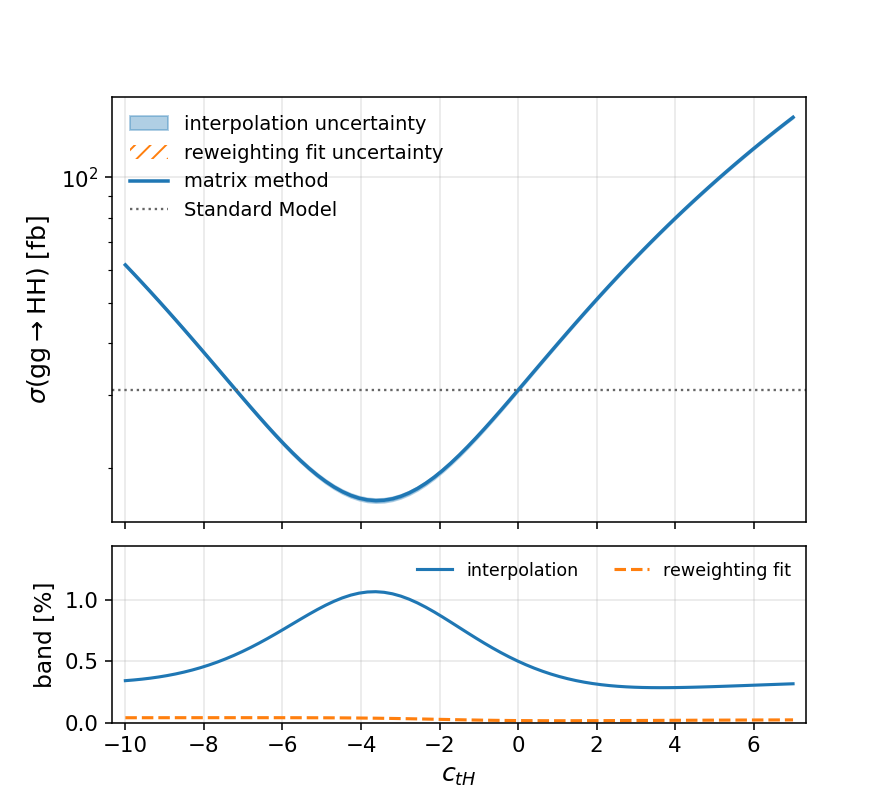
\includegraphics[width=0.40\textwidth]{figures/basis_optimization/unc_yield_ctH.png}
    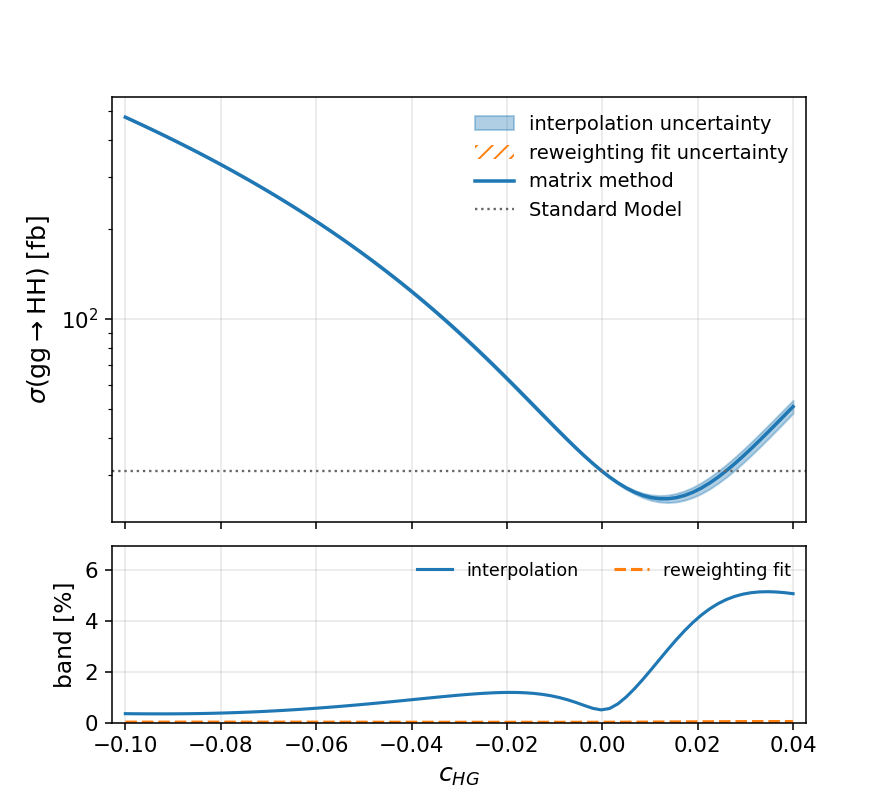
\includegraphics[width=0.40\textwidth]{figures/basis_optimization/unc_yield_cHG.png}\\
    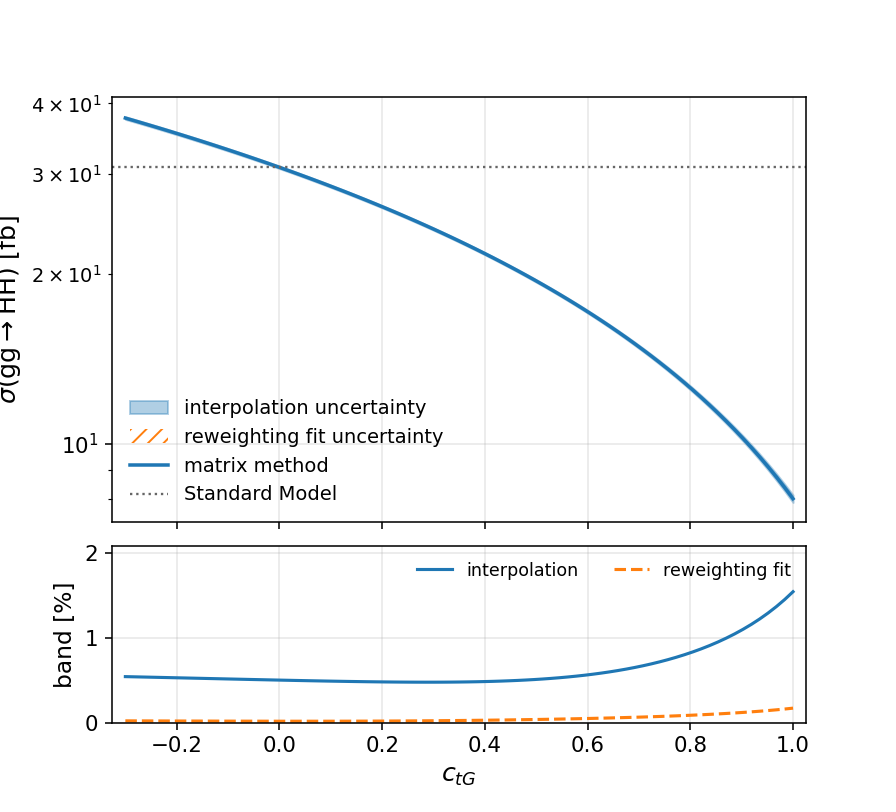
\includegraphics[width=0.40\textwidth]{figures/basis_optimization/unc_yield_ctG.png}
    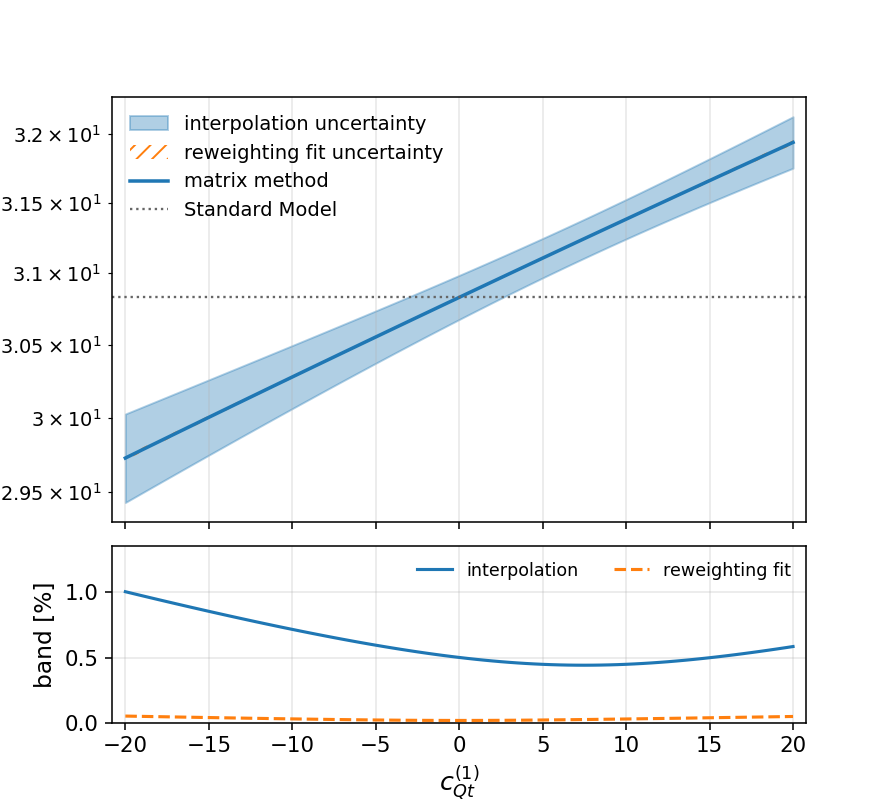
\includegraphics[width=0.40\textwidth]{figures/basis_optimization/unc_yield_cQt1.png}
    \caption{Scans along $c_{\PQt\PH}$, $c_{\PH G}$, $c_{\PQt G}$ and
    $c_{Q\PQt}^{(1)}$.}
    \label{fig:unc_yield_extra1}
\end{figure}

\begin{figure}[htbp]
    \centering
    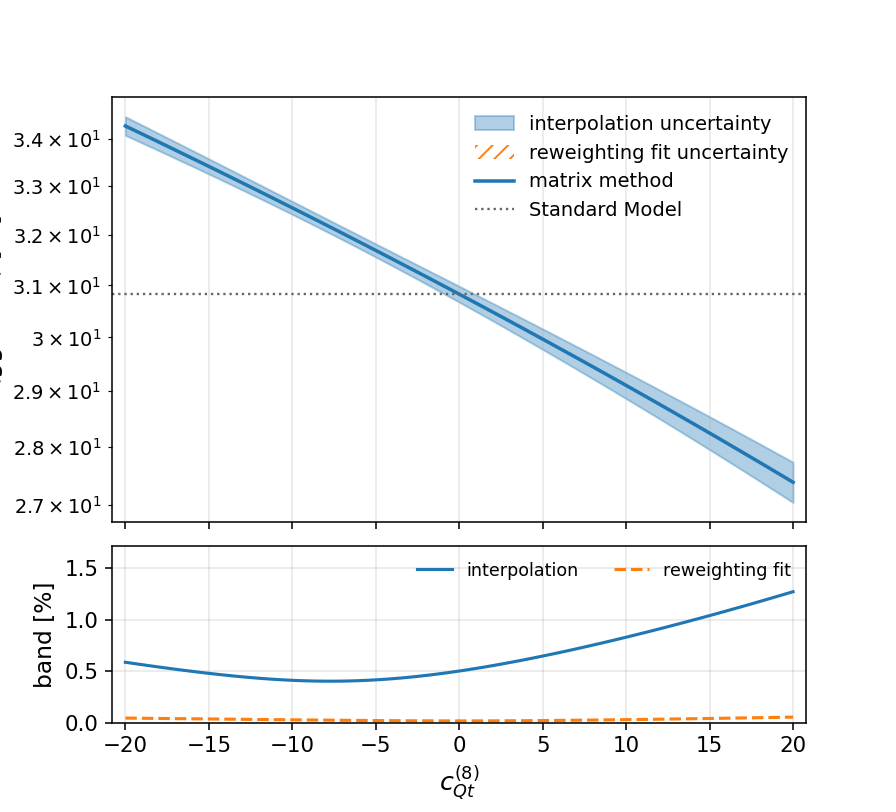
\includegraphics[width=0.40\textwidth]{figures/basis_optimization/unc_yield_cQt8.png}
    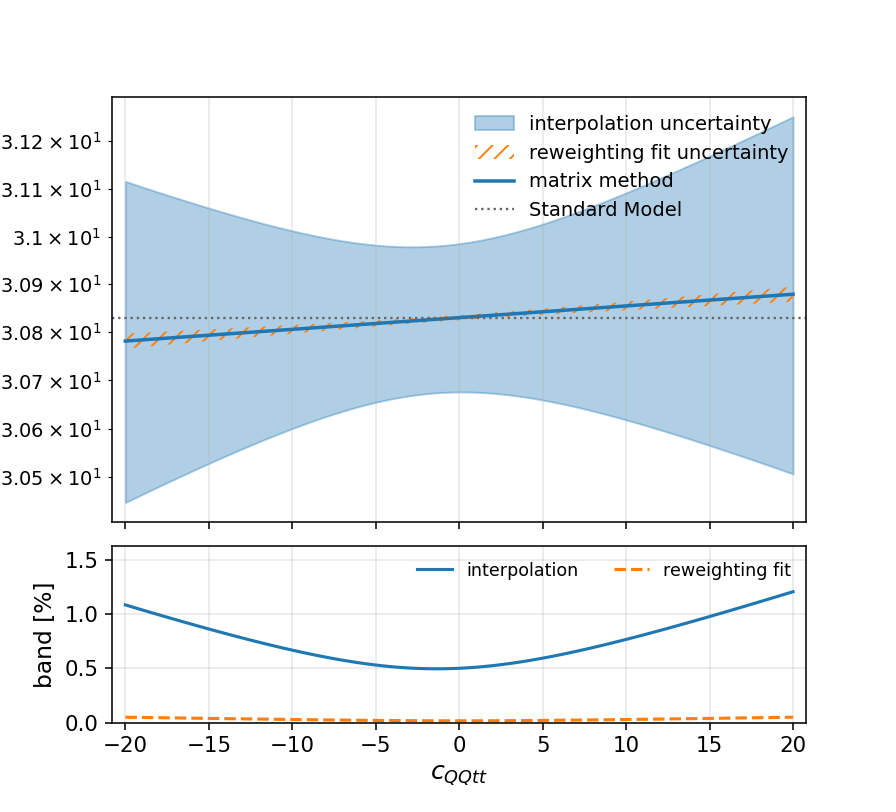
\includegraphics[width=0.40\textwidth]{figures/basis_optimization/unc_yield_cQQtt.png}\\
    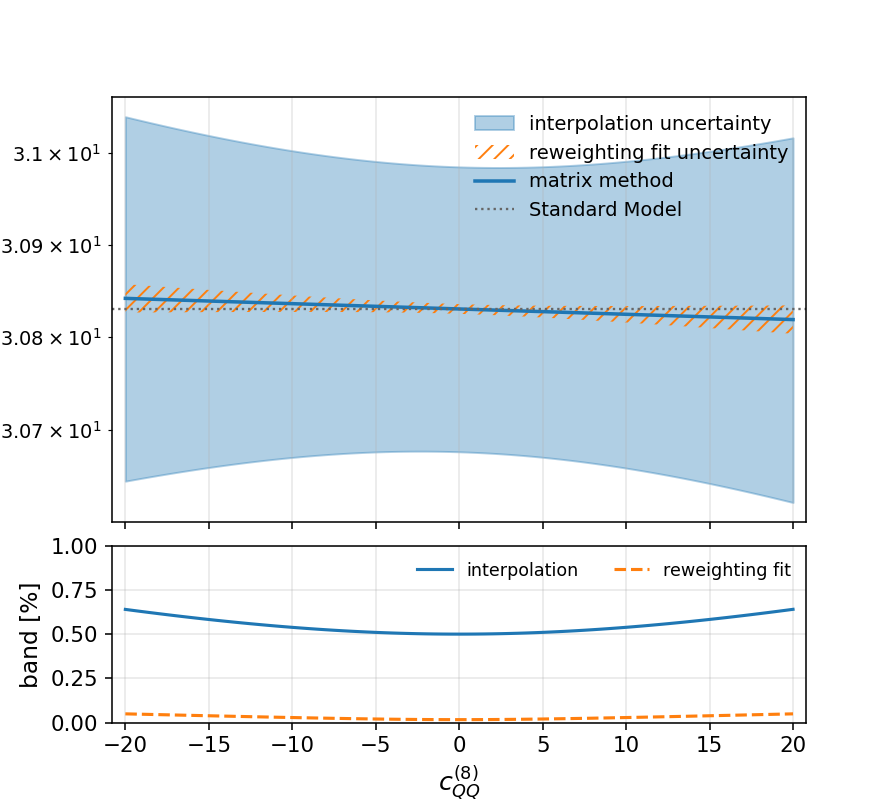
\includegraphics[width=0.40\textwidth]{figures/basis_optimization/unc_yield_cQQ8.png}
    \caption{Scans along $c_{Q\PQt}^{(8)}$, $c_{QQ\PQt\PQt}$ and $c_{QQ}^{(8)}$.}
    \label{fig:unc_yield_extra2}
\end{figure}

\begin{table}[htbp]
\centering
\begin{tabular}{l|cc|cc}
\hline
 & \multicolumn{2}{c|}{band, fraction of the yield} &
   \multicolumn{2}{c}{scanned range} \\
coefficient & smallest & largest & from & to \\
\hline
$c_{\PH}$               & $0.2\%$ & $5.8\%$ & $-50$   & $50$   \\
$c_{\PH\mathrm{kin}}$   & $0.3\%$ & $0.7\%$ & $-8$    & $8$    \\
$c_{\PQt\PH}$           & $0.3\%$ & $1.1\%$ & $-10$   & $7$    \\
$c_{\PH G}$             & $0.3\%$ & $5.1\%$ & $-0.1$  & $0.04$ \\
$c_{\PQt G}$            & $0.5\%$ & $1.5\%$ & $-0.3$  & $1$    \\
$c_{Q\PQt}^{(1)}$       & $0.4\%$ & $1.0\%$ & $-20$   & $20$   \\
$c_{Q\PQt}^{(8)}$       & $0.4\%$ & $1.3\%$ & $-20$   & $20$   \\
$c_{QQ\PQt\PQt}$        & $0.5\%$ & $1.2\%$ & $-20$   & $20$   \\
$c_{QQ}^{(8)}$          & $0.5\%$ & $0.6\%$ & $-20$   & $20$   \\
\hline
\end{tabular}
\caption{Range of the interpolation uncertainty as a fraction of the predicted
yield, over each one-dimensional scan. Every scan passes through $0.50\%$ at the
SM.}
\label{tab:unc_bands}
\end{table}

\begin{table}[htbp]
\centering
\begin{tabular}{l|cc}
\hline
plane & median $|\Delta|/|\Delta|_\mathrm{stat}$ & bins with $|$pull$|<1$ \\
\hline
$c_{\PH}$--$c_{\PQt\PH}$                 & $0.74$ & $0.72$ \\
$c_{\PH}$--$c_{\PH G}$                   & $0.71$ & $0.74$ \\
$c_{\PH}$--$c_{\PQt G}$                  & $0.71$ & $0.67$ \\
$c_{\PH\mathrm{kin}}$--$c_{\PQt\PH}$     & $0.88$ & $0.71$ \\
$c_{Q\PQt}^{(1)}$--$c_{QQ}^{(8)}$        & $0.65$ & $0.76$ \\
\hline
\end{tabular}
\caption{Size of the interpolation uncertainty against the residual actually
observed, per plane of the generated grid. The first column is the median over
the plane of the ratio defined in Sec.~\ref{sec:uncertainties}, the second the
fraction of bins whose pull is within one standard deviation; a standard normal
gives $0.683$.}
\label{tab:unc_calibration}
\end{table}

\subsection{The modelling uncertainty per selection}
\label{sec:appendix_unc_per_selection}
\label{sec:appendix_unc_realistic}

The two terms that make up $\sigma_\mathrm{mod}$ are given separately in
Tab.~\ref{tab:unc_components}. Which of them dominates is not a property of the
method but of the selection and the coefficient: $\sigma_\mathrm{ELR}$ is the
larger in the resolved selection for every coefficient, and in the merged one
for four of the six, while for $c_{\PH G}$ in the merged selection the ordering
inverts, that being where the merged templates are thinnest. The composition of one
entry therefore does not carry to the others.

\begin{table}[htbp]
\centering
\begin{tabular}{l|ccc|ccc}
\hline
 & \multicolumn{3}{c|}{$4\PQb$ resolved} & \multicolumn{3}{c}{$4\PQb$ fully merged} \\
coefficient & $\sigma_\mathrm{MM}$ & $\sigma_\mathrm{ELR}$ & $\sigma_\mathrm{mod}$ & $\sigma_\mathrm{MM}$ & $\sigma_\mathrm{ELR}$ & $\sigma_\mathrm{mod}$ \\
\hline
$c_\PH$                & $0.20\%$ & $0.49\%$ & $0.53\%$ & $1.48\%$ & $3.39\%$ & $3.77\%$ \\
$c_{\PH\mathrm{kin}}$  & $0.17\%$ & $1.14\%$ & $1.16\%$ & $1.20\%$ & $1.73\%$ & $2.01\%$ \\
$c_{\PQt\PH}$          & $0.22\%$ & $0.96\%$ & $0.98\%$ & $1.17\%$ & $1.47\%$ & $1.86\%$ \\
$c_{\PH G}$            & $0.28\%$ & $0.97\%$ & $1.02\%$ & $2.76\%$ & $0.62\%$ & $2.85\%$ \\
$c_{\PQt G}$           & $0.14\%$ & $1.50\%$ & $1.50\%$ & $0.99\%$ & $3.03\%$ & $3.17\%$ \\
$c_{Q\PQt}^{(1)}$      & $0.20\%$ & $0.63\%$ & $0.65\%$ & $1.94\%$ & $1.40\%$ & $2.33\%$ \\
\hline
\end{tabular}
\caption{The two terms of the modelling uncertainty of
Fig.~\ref{fig:unc_realistic_cH}, as a fraction of the predicted yield, at the
median of each one-dimensional scan with the other eight coefficients at zero.
$\sigma_\mathrm{MM}$ is the Monte Carlo statistical error of the basis
templates propagated through the morphing weights, $\sigma_\mathrm{ELR}$ the
uncertainty of the reweighting coefficients the templates were made with, and
$\sigma_\mathrm{mod}^2=\sigma_\mathrm{MM}^2+\sigma_\mathrm{ELR}^2$ the quantity
drawn in the lower panel of those figures. The weights are the same in both
pairs of columns; the template errors are each selection's own.}
\label{tab:unc_components}
\end{table}

The six scans of Sec.~\ref{sec:validation_realistic_band} follow, in a common format:
the predicted yield after the resolved and the fully merged selection along one Wilson
coefficient, with the modelling uncertainty $\sigma_{\text{mod}}$ of
Eq.~\eqref{eq:sigmainterp} combined with the reweighting term as a band, and the band size as a fraction of the yield in the
lower pad.

\begin{figure}[htbp]
    \centering
    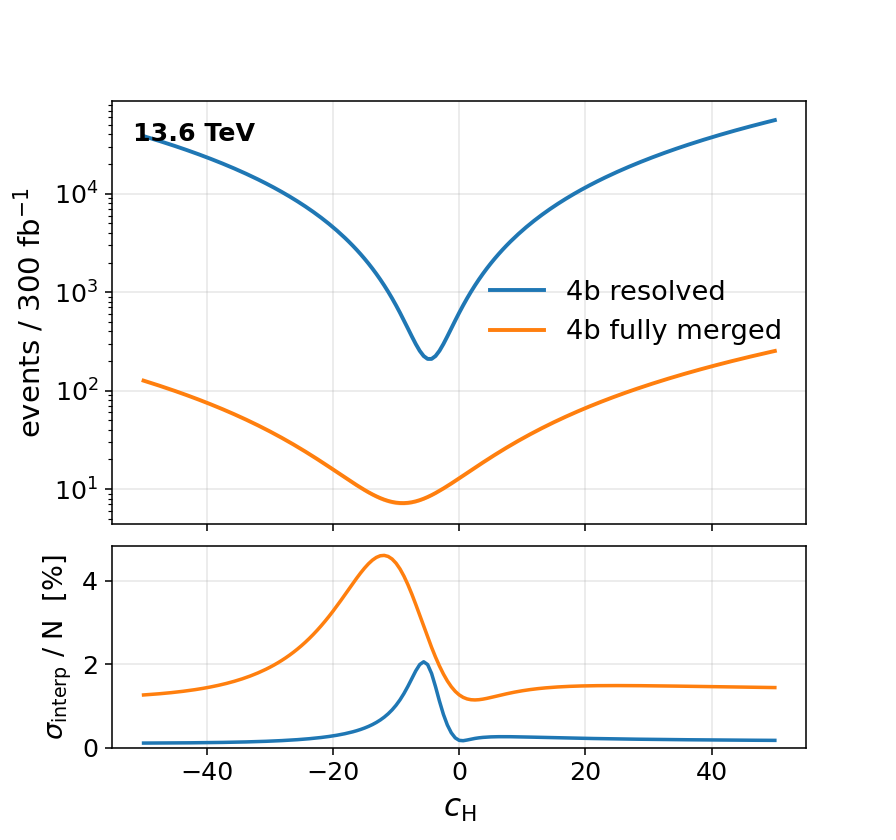
\includegraphics[width=0.52\textwidth]
        {figures/basis_optimization/realistic_unc_cH.png}
    \caption{Predicted yield after the resolved and the fully merged
    $\HH\to\bbbar\bbbar$ selections along $c_{\PH}$, with the modelling uncertainty as a
    band; lower pad, the band size as a fraction of the yield.}
    \label{fig:unc_realistic_cH}
\end{figure}

\begin{figure}[htbp]
    \centering
    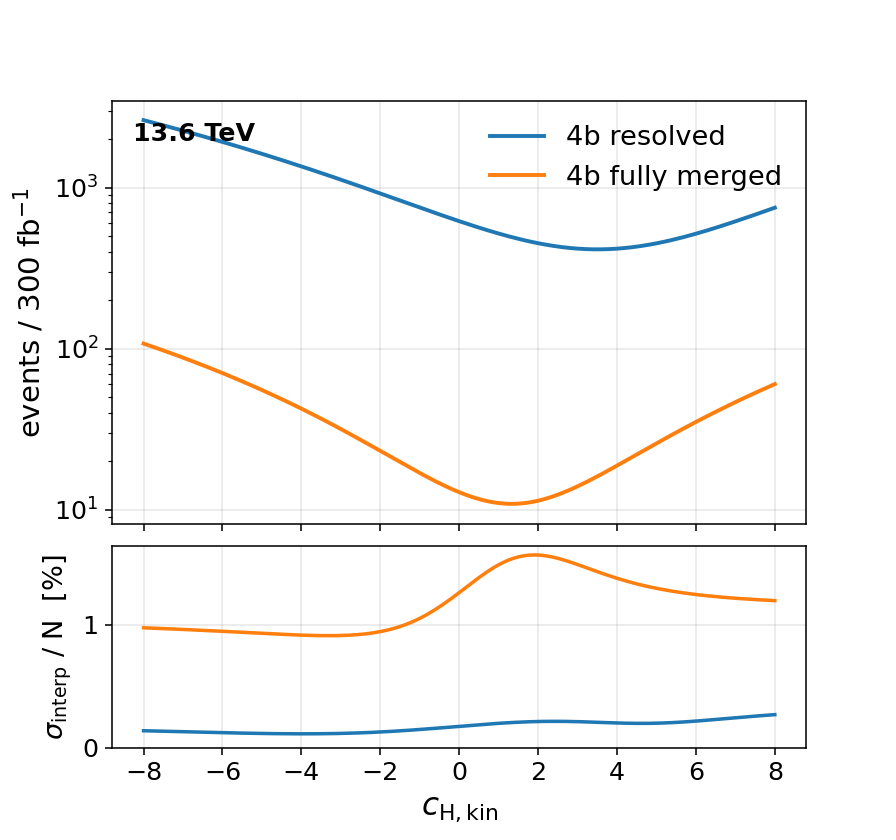
\includegraphics[width=0.52\textwidth]
        {figures/basis_optimization/realistic_unc_cHkin.png}
    \caption{The same quantities as in Fig.~\ref{fig:unc_realistic_cH}, along
    $c_{\PH\mathrm{kin}}$.}
    \label{fig:unc_realistic_cHkin}
\end{figure}

\begin{figure}[htbp]
    \centering
    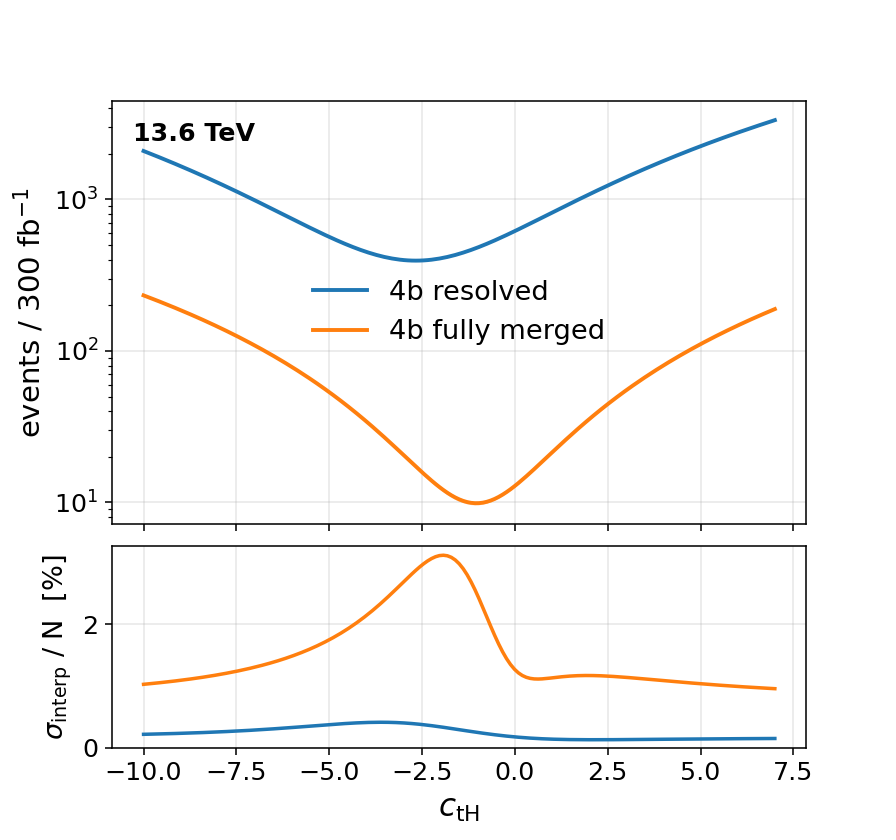
\includegraphics[width=0.52\textwidth]
        {figures/basis_optimization/realistic_unc_ctH.png}
    \caption{The same quantities as in Fig.~\ref{fig:unc_realistic_cH}, along
    $c_{\PQt\PH}$.}
    \label{fig:unc_realistic_ctH}
\end{figure}

\begin{figure}[htbp]
    \centering
    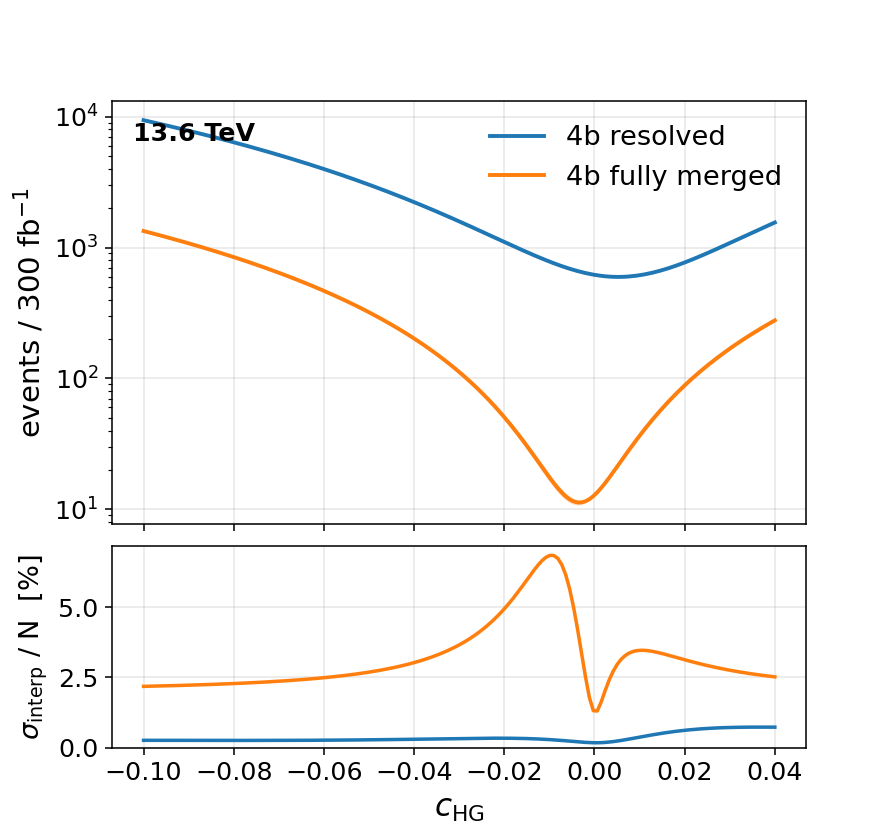
\includegraphics[width=0.52\textwidth]
        {figures/basis_optimization/realistic_unc_cHG.png}
    \caption{The same quantities as in Fig.~\ref{fig:unc_realistic_cH}, along
    $c_{\PH G}$.}
    \label{fig:unc_realistic_cHG}
\end{figure}

\begin{figure}[htbp]
    \centering
    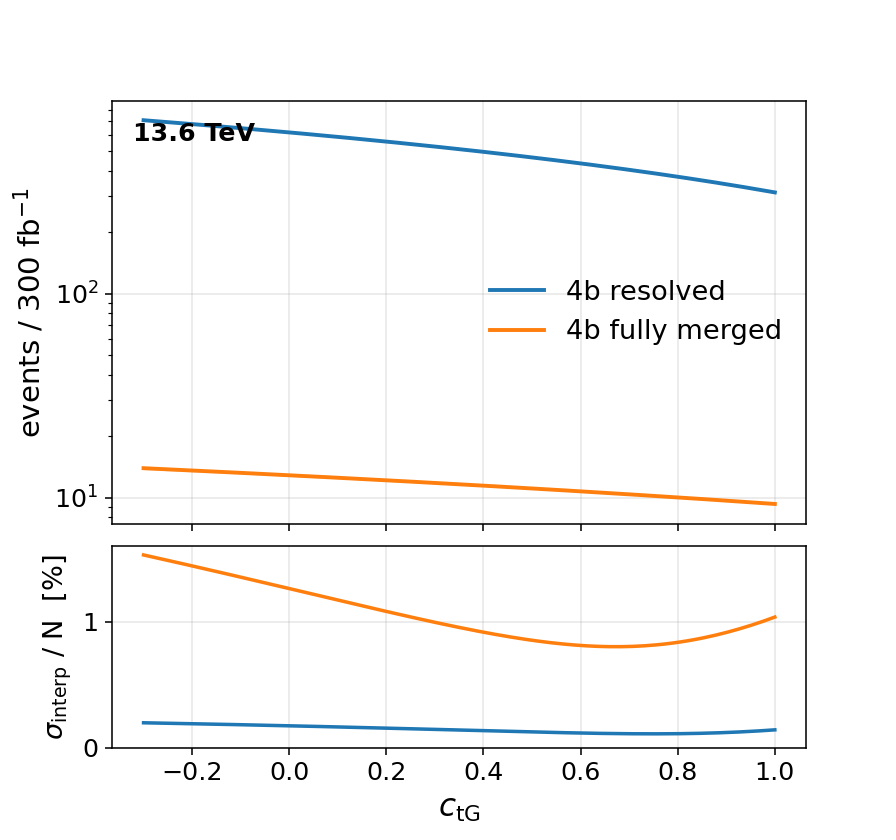
\includegraphics[width=0.52\textwidth]
        {figures/basis_optimization/realistic_unc_ctG.png}
    \caption{The same quantities as in Fig.~\ref{fig:unc_realistic_cH}, along
    $c_{\PQt G}$.}
    \label{fig:unc_realistic_ctG}
\end{figure}

\begin{figure}[htbp]
    \centering
    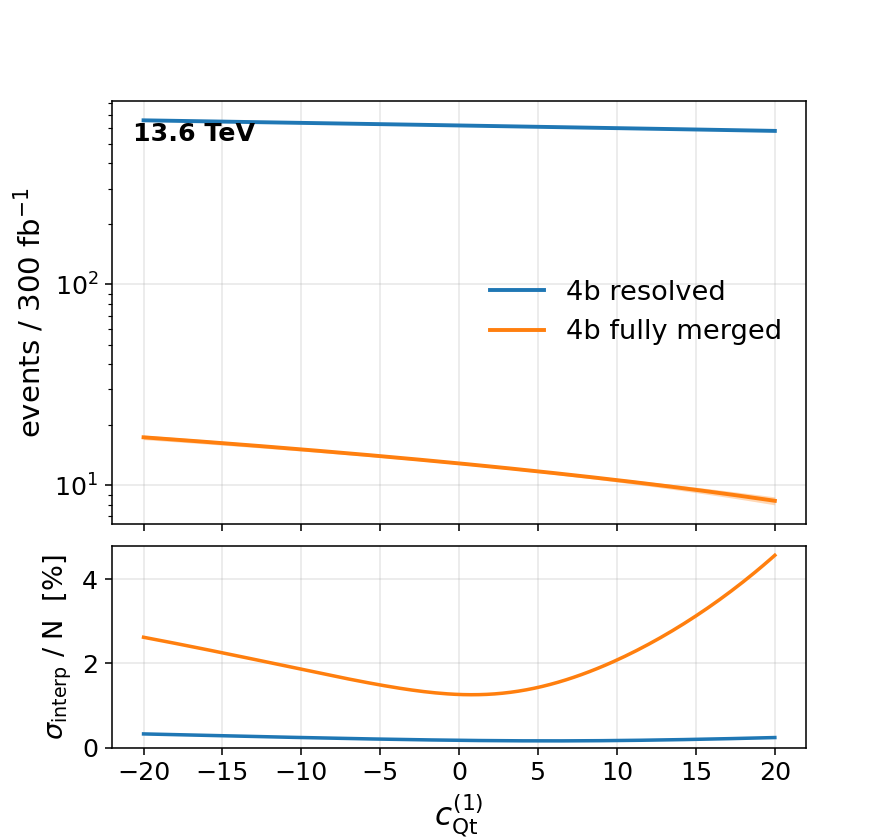
\includegraphics[width=0.52\textwidth]
        {figures/basis_optimization/realistic_unc_cQt1.png}
    \caption{The same quantities as in Fig.~\ref{fig:unc_realistic_cH}, along
    $c_{Q\PQt}^{(1)}$.}
    \label{fig:unc_realistic_cQt1}
\end{figure}

For reference, the same band evaluated on the inclusive cross section, with no
selection applied, is shown below. It is one band rather than two because there
is one set of $\sigma_i$; this is the figure that
Sec.~\ref{sec:validation_realistic_band} replaces with a measurement.

\begin{figure}[htbp]
    \centering
    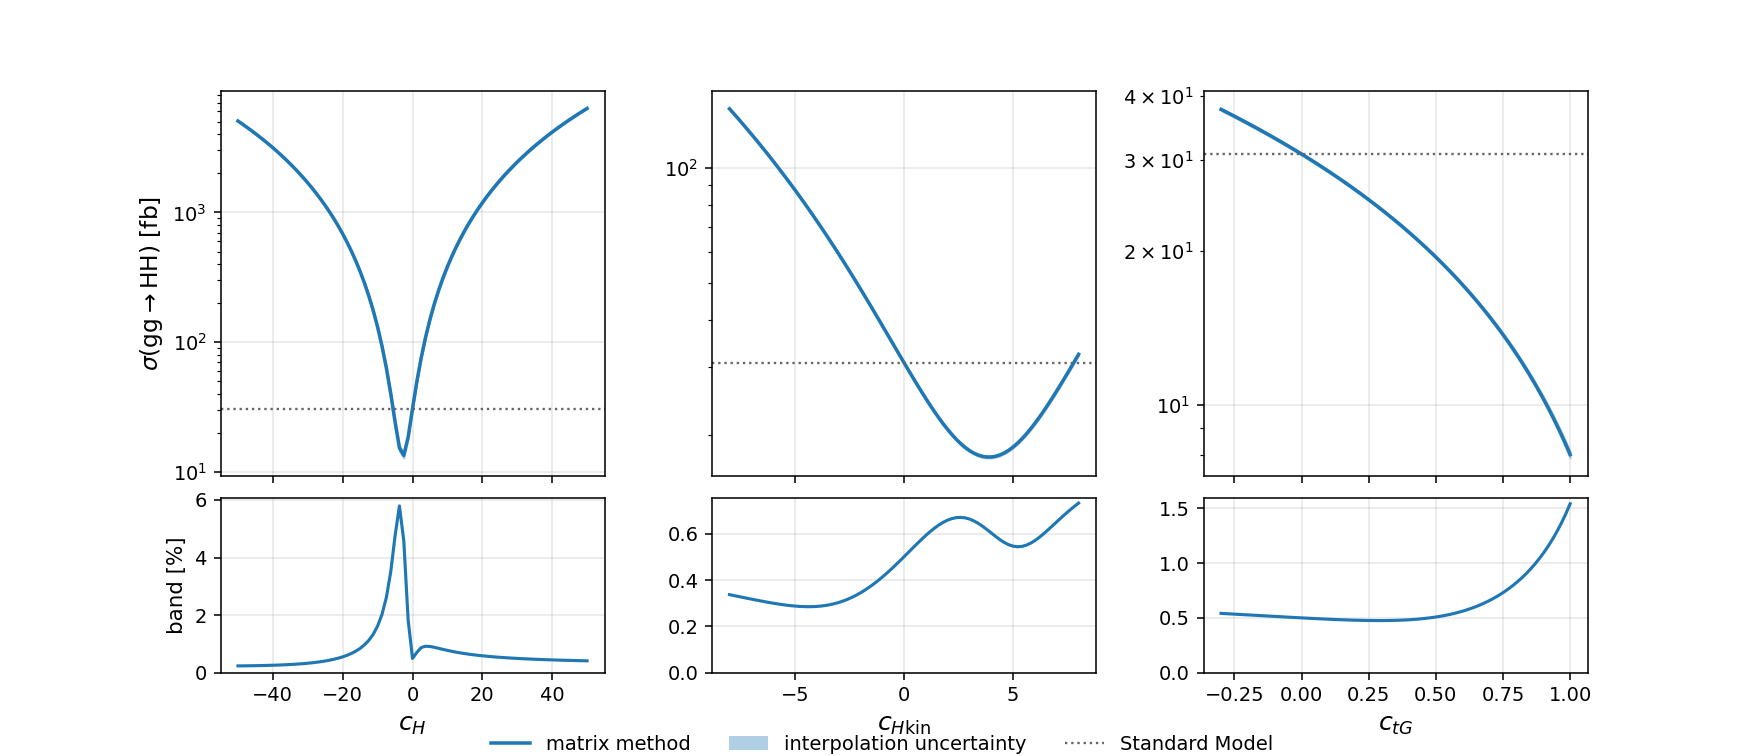
\includegraphics[width=\textwidth]
        {figures/basis_optimization/unc_yield_row.png}
    \caption{Predicted \ggHH cross section along $c_\PH$, $c_{\PH\mathrm{kin}}$
    and $c_{\PQt G}$, in each case with the other eight coefficients at zero,
    with the interpolation uncertainty of Eq.~\eqref{eq:sigmainterp}. The dotted
    line is the SM. The lower panels repeat the uncertainty as a
    fraction of the yield. Note the different vertical scales.}
    \label{fig:unc_yield}
\end{figure}

\subsection{\textcolor{red}{[AUTHORS ONLY]} The same uncertainty in the HEFT basis}
\label{sec:appendix_heft_unc}

\textcolor{red}{This subsection is for the authors and is not intended for the
published version. It is here to record that the prescription is not specific to the
SMEFT parameterization, and to give the numbers for the HEFT basis before deciding
whether any of it belongs in the report.}

Nothing in Eq.~\eqref{eq:sigmainterp} refers to SMEFT. It needs a basis, the
parameterization the weights are solved from, and the statistical errors of the
templates. Replacing the forty SMEFT monomials by the twenty-three of the
$\kappa$-framework HEFT parameterization in $\kappa_\lambda$, $\kappa_\PQt$, $c_2$,
$c_g$ and $c_{2g}$, and applying the same weights to the same two $4\PQb$ selections,
gives Table~\ref{tab:unc_heft}. The basis is the published twenty-three-point HEFT set,
square and of condition number $1.0\times10^{4}$, against $1.9\times10^{6}$ for the
forty-point SMEFT one.

The templates and their covariance are recomputed here from the input trees of the two
$4\PQb$ selections, one pass per input sample carrying every basis point's weight, so
the band can be given in both forms: the exact one, $\sqrt{w^{T}Sw}$ with the full
covariance of Eq.~\eqref{eq:sigmaMMcov}, and the independent one of
Eq.~\eqref{eq:sigmainterp}. The merged selection costs a factor five to eight over the
resolved one, as in the SMEFT case. The two forms differ most along $c_{2g}$, the
direction the twenty-three points constrain least: there the independent form gives
$3.54\%$ in the median and $9.49\%$ at its largest in the merged selection, against
$1.90\%$ and $2.04\%$ exactly, so the band that looked an order of magnitude worse than
the others is mostly the correlation between templates, counted twice. Bin by bin the
ratio of the two forms runs from $0.7$ to about $35$. At the SM the exact band is
$0.173\%$ of the resolved yield and $1.27\%$ of the merged one.

\textcolor{red}{Produced with \texttt{scripts/gghh\_smeft/mm\_covariance\_from\_trees.py}
and \texttt{mm\_covariance\_scans.py} of the toolkit, which reproduce the
\texttt{ELReweighter} templates in numpy: the integrated yields of the twenty-three basis
points agree with the delivered table to $0.1\%$ in the median (resolved).}

\textcolor{red}{The earlier version of this table, and the $18\%$ it quoted on $c_{2g}$,
came from the \texttt{err\_yield} column of that delivered table and should not be
quoted. That column is a factor $\simeq\sqrt{2}$ above the inverse-variance combination
of the same four inputs, uniformly over the twenty-three points and both regions
($0.70\pm0.03$). The card side reproduced the same ratio with the \texttt{ELReweighter}
itself, so the factor is in the table and not in the templates: the table was committed
from an external production and is written by no script of the package, and a doubled
\texttt{Sumw2} at filling or merging would produce exactly that flat factor. The numbers
above are built from the events and do not depend on it, and the SMEFT tables used
elsewhere in this report are written by \texttt{make\_datacards} from the same templates
the card uses, with errors equal to $\sqrt{S_{ii}}$ and no such factor --- consistently,
the resolved band at the SM is $0.17\%$ there as it is here.}

\begin{table}[htbp]
\centering
\begin{tabular}{l|cc|cc|cc|cc}
\hline
 & \multicolumn{4}{c|}{$4\PQb$ resolved} & \multicolumn{4}{c}{$4\PQb$ fully merged} \\
 & \multicolumn{2}{c|}{exact} & \multicolumn{2}{c|}{independent}
 & \multicolumn{2}{c|}{exact} & \multicolumn{2}{c}{independent} \\
coupling & median & largest & median & largest & median & largest & median & largest \\
\hline
$\kappa_\lambda$ & $0.20\%$ & $0.24\%$ & $0.21\%$ & $0.50\%$ & $1.37\%$ & $1.68\%$ & $1.48\%$ & $1.82\%$ \\
$\kappa_\PQt$    & $0.17\%$ & $0.19\%$ & $0.22\%$ & $0.38\%$ & $1.27\%$ & $1.27\%$ & $1.21\%$ & $1.23\%$ \\
$c_2$            & $0.22\%$ & $0.28\%$ & $0.23\%$ & $0.65\%$ & $1.36\%$ & $1.41\%$ & $1.49\%$ & $4.71\%$ \\
$c_g$            & $0.17\%$ & $0.18\%$ & $0.24\%$ & $0.34\%$ & $1.27\%$ & $1.27\%$ & $1.20\%$ & $2.54\%$ \\
$c_{2g}$         & $0.26\%$ & $0.43\%$ & $0.38\%$ & $0.50\%$ & $1.90\%$ & $2.04\%$ & $3.54\%$ & $9.49\%$ \\
\hline
\end{tabular}
\caption{\textcolor{red}{[AUTHORS ONLY]} Interpolation uncertainty as a fraction of the
predicted yield, median and largest over each one-dimensional scan, for the
twenty-three-point HEFT basis and the two $4\PQb$ selections of Ref.~\cite{CMS:2026znu}.
``Exact'' is $\sqrt{w^{T}Sw}$ with the full covariance of the templates,
Eq.~\eqref{eq:sigmaMMcov}; ``independent'' is Eq.~\eqref{eq:sigmainterp}, its diagonal.
Both are built from the same templates, summed over \mHH. The other four couplings are
at their SM values in each scan. Ranges scanned: $\kappa_\lambda\in[-10,15]$,
$\kappa_\PQt\in[0.5,1.75]$, $c_2\in[-1,1.5]$, $c_g,c_{2g}\in[-0.6,0.6]$.}
\label{tab:unc_heft}
\end{table}

\textcolor{red}{Not done, and the reason: the same table for \ggHHH and $\PQt\PAQt\HH$
cannot be produced from what exists. Their bases load and solve --- the run-2 \ggHHH
set is nine points for nine monomials, the $\PQt\PAQt\HH$ one six points for three and
therefore over-determined, needing a least-squares solve --- but none of the \ggHHH or
$\PQt\PAQt\HH$ yield tables carries a per-template statistical error, which is the one
input the method cannot do without. One extra column per region from whatever produced
those tables would close it. The \ggHH HEFT numbers above exist precisely because those
tables do carry it.}

\textcolor{red}{\textbf{SPYROS:} items (i) and (ii) below are built and checked on the
card side; (iii) is still open.
\textbf{(i)} The per-bin template covariance $S_j$, with
$S_{j,ik}=\sum_s \alpha_{sj}(i)\,\alpha_{sj}(k)\,C_{s,j,ik}$, is produced by the
\texttt{ELReweighter} and read by the physics model, which builds one nuisance parameter
per channel of size $\sigma_j(\mathbf{c})/N_j(\mathbf{c})$ with
$\sigma_j^2=\phi^{T}(A^{T}S_jA)\phi$ a polynomial in the couplings, so the size follows
the parameters of interest. Checked against the same quantity computed outside the workspace to
$4\times10^{-13}$ over six points and twenty-three channels. The comparison asked for
--- $\sqrt{w^{T}S_jw}$ against $\sqrt{\sum_i w_i^2 S_{j,ii}}$ --- is in the table above
and in Sec.~\ref{sec:uncertainties}: the off-diagonal is not a refinement.
\textbf{(ii)} Cards written with one channel per \mHH bin, so the uncertainty enters as
a rate scaling per bin through \texttt{getYieldScale}. Without shape nuisances the
likelihood is identical, checked at $3.5\times10^{-9}$ in $-2\Delta\ln L$ on the
\HHbbbb example; a shape nuisance such as \texttt{CMS\_reweight} keeps its name in every
channel and acts per bin as a log-normal, which costs $0.065$ in $-2\Delta\ln L$ at a
value of about $340$. \texttt{autoMCStats} becomes per bin and covers the background
only: Combine leaves signal processes out of it unless its include-signal field is set,
and the cards do not set it, so the morphed signal's Monte Carlo statistics are carried
by the nuisance of (i) and by nothing else.
\textbf{(iii)} The \texttt{err\_yield} column above, for \ggHHH and
$\PQt\PAQt\HH$, which only completes this table.}

\clearpage
\subsection{\textcolor{red}{[AUTHORS ONLY]} Restricted morphing: the HEFT checks and the timing}
\label{sec:appendix_slices_heft}

\textcolor{red}{This subsection is for the authors and is not intended for the published
version. It records that the restriction of Sec.~\ref{sec:slice_models} is not specific
to SMEFT, keeps the timing measurements that are quoted only as an order of magnitude in
the main text, and records why the closure figures behind those numbers are not
shown.}

\textcolor{red}{\textbf{Why there are no figures here.} The exactness checks were run on
a mock statistical model: the \HHbbbb example card uses an invented, strictly falling
background, chosen so that the fits would run at all, not so that they would mean
anything. The scans and contours it produces are therefore not physics results and must
not be shown, in the report or elsewhere. The \emph{comparison} between the restricted
and the full model is unaffected by it: both see the same background and only the
difference between them is read off. Only those differences are quoted.}

\paragraph{HEFT.} Nothing in the construction refers to SMEFT. The restriction needs a
polynomial prediction and morphing weights that are polynomials in the same monomials,
which is as true of the HEFT parameterization as of the $40$-term SMEFT one.
Run on a counting-experiment multilepton example with the five-coefficient HEFT basis,
the restricted and full models agree to better than $3\times10^{-7}$ in
$-2\Delta\ln L$ in every case tested: $\kappa_\lambda$ alone; $\kappa_\lambda \times
\kappa_{\PQt}$ in two dimensions; $\kappa_\lambda$ with $\kappa_{\PQt}$ fixed away from
its SM value; $\kappa_\lambda$ with $\kappa_{\PQt}$ profiled; and
$\kappa_\lambda$ with $\kappa_{\PQt}$, $c_2$, $c_g$ and $c_{2g}$ added to the profiled
set one at a time. A scan in $\kappa_\lambda$ alone keeps $4$ of the $24$ templates.

\paragraph{SMEFT, in detail.} On the nine-coefficient Warsaw-Higgs basis with the
\HHbbbb shape card ($23$ \mHH bins), the agreement in $-2\Delta\ln L$ between the
restricted and the full model is below $10^{-9}$ with nothing profiled ($5\times10^{-7}$
for the two-dimensional scan), below $2\times10^{-5}$ with up to three coefficients
profiled, and below $2\times10^{-3}$ with four, five or seven. With six and with all
eight profiled it is $0.4$; with all eight the restricted model keeps all $40$ templates
and \emph{is} the full model, so that number is the minimiser's own spread with eight
free directions on one shape card, not an effect of the restriction.

\paragraph{Timing.} Measured on one realistic analysis model, one scan point, the same
minimiser settings, one core each, side by side on one machine. The analysis is not
named and these are order-of-magnitude figures only.

\begin{table}[htbp]
\centering
\begin{tabular}{l|c|c}
\hline
statistical model & \HH signal templates & one scan point \\
\hline
a few templates, no systematic uncertainties      & $6$  & $\sim 0.5$~min \\
SM-like $\kappa$ model, full systematics & $18$ & $\sim 9$~min \\
nine-coefficient basis, full systematics          & $80$ & $\sim 30$~min \\
\quad restricted to $c_{\PH\mathrm{kin}}$, full systematics & $12$ & $\sim 6$~min \\
\hline
\end{tabular}
\caption{\textcolor{red}{[AUTHORS ONLY]} Cost of one likelihood scan point against the
number of \HH signal templates in the model. The restriction returns about a factor five.
On the public \HHbbbb example the difference is not resolved --- $8$--$10$~s for a
$33$-point scan either way, dominated by start-up.}
\label{tab:slices_timing}
\end{table}

\paragraph{Minimiser settings.} The exactness checks above used strategy $1$ and
tolerance $0.001$ throughout. \textcolor{red}{This paragraph previously reported that
with strategy $0$ and tolerance $0.1$ the full model failed to converge where the
restricted one did --- at $c_{\PH}=19.5$ with $c_{\PH\mathrm{kin}}$ profiled it
returned $-2\Delta\ln L = 949$ against the converged $1478$. That reading is withdrawn:
the scatter it rested on was traced on the card side to the expected dataset differing
from fit to fit, not to the size of the model, and the likelihood of the full model was
then found to be smooth and its minimisation reproducible and independent of the
settings. The case for the restriction is cost and exactness.}

\clearpage
\subsection{\textcolor{red}{[AUTHORS ONLY]} Checks on the energy transport}
\label{sec:appendix_energy_checks}

\textcolor{red}{This subsection is for the authors. The three panels below were used to
build and check the transported coefficient files; none of them is required by an
argument in the main text, which quotes the numbers directly.
Panel (c) is now in the main text, as the right
panel of Fig.~\ref{fig:energy_transport}, since the statement it carries --- that the
tail residual belongs to the kernel and not to the direction of the step --- is used
there to set the $14$~TeV shape uncertainty. It is repeated here only because the three
panels come from one file. \textbf{Decide whether to keep (a) and (b):} they verify the
kernel that is written into the released files.}

\begin{figure}[htbp]
\centering
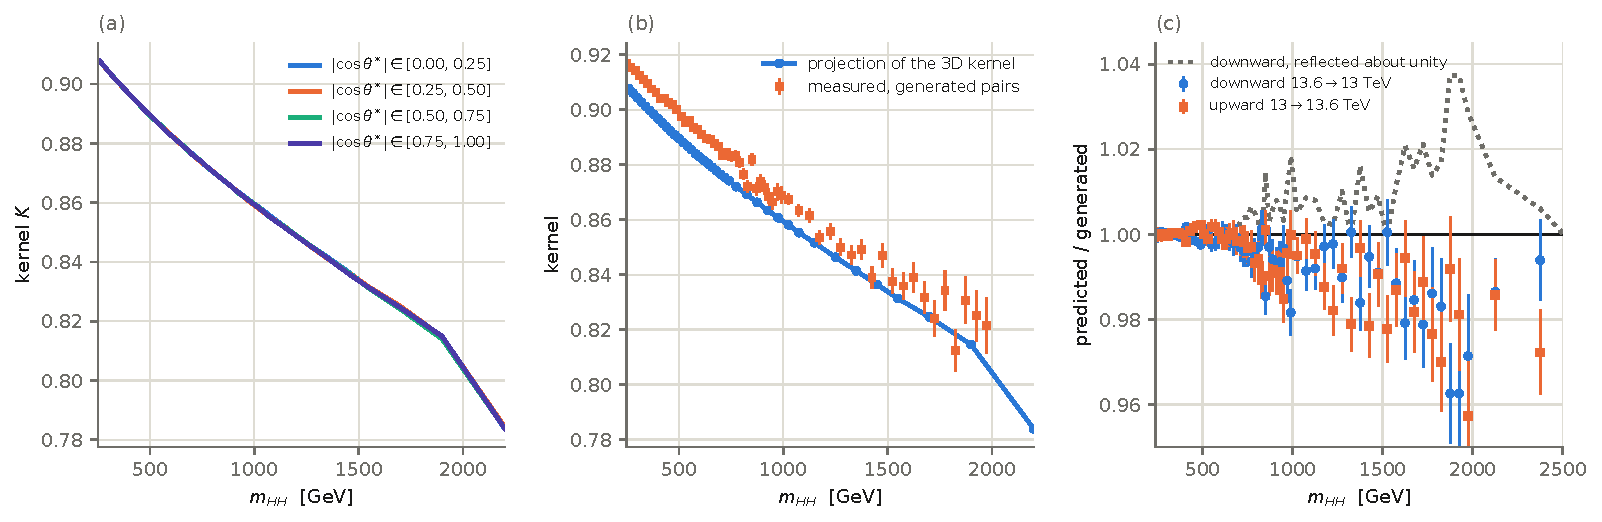
\includegraphics[width=\linewidth]{plots/energy_transport_checks.pdf}
\caption{\textcolor{red}{[AUTHORS ONLY]} Checks on the $13$~TeV transport.
(a) The per-bin kernel written into the coefficient file, split by $|\cos\theta^*|$.
(b) Its projection onto \mHH against the kernel measured from the 2784 generated pairs.
(c) The transport run in both directions over the same step in $\ln\sqrt{s}$, each
anchored on its own constant; the dotted curve is the downward result reflected about
unity.}
\label{fig:energy_checks}
\end{figure}

Panel (a) shows the kernel to be independent of $|\cos\theta^*|$ to within the line
width, so the transport is a function of \mHH alone at the present statistics. Panel (b)
shows its projection reproducing the independently measured kernel with the $1\%$ offset
quoted in Sec.~\ref{sec:energy_transport}. In panel (c) the overall constant inverts
between the two directions, $1.0098$ against $1/0.9902 = 1.0099$, while the per-bin
residual stays negative in both: anchored mean pulls are $-0.8$, $-1.2$, $-1.8$ and
$-0.6$ downward across the bands below $1$~TeV, $1$--$1.5$, $1.5$--$2$ and above
$2$~TeV, against $-0.4$, $-1.7$, $-1.8$ and $-2.5$ upward.

\clearpage
\subsection{\textcolor{red}{[AUTHORS ONLY]} Single-Higgs scaling with \texorpdfstring{$c_\PH$}{cH}: the implementation}
\label{sec:appendix_singleh}

\textcolor{red}{This subsection is for the authors and is not intended for the published
version. \textbf{Nothing in it is a new result.} Every curve here was produced with our
own implementation of scalings that already exist in the literature --- the $C_1$
coefficients and the $\kappa_\lambda$ dependence of single-Higgs production and decay
(Refs.~\cite{Degrassi:2016wml,Maltoni:2017ims}), including their use per STXS bin
(Refs.~\cite{ATLAS:2024lyh,Brivio:2022pyi}). The subsection exists for one purpose: to
let us check that our implementation reproduces what those references and the internal
CMS single-Higgs fits already give, before any of it is used. If a number here disagrees
with the literature, the implementation is wrong, not the literature. The two statements
that \emph{are} specific to this report --- the physical region of
$c_{\PH\mathrm{kin}}$ and the truncation of $\sigma\times\mathrm{BR}$ --- are in
Secs.~\ref{sec:trunc_singleh} and~\ref{sec:trunc_product}, and are not repeated here.}

The nine Wilson coefficients of Eq.~\eqref{eq:smeftpoint} also enter single-Higgs
production and decay, and a global fit constrains them with single-\PH and \HH data
together. Single-Higgs measurements are interpreted through the
STXS~\cite{Berger:2019wnu,deFlorian:2016spz}, bins in production
mode and a few kinematic variables, each parameterized as a polynomial in the Wilson
coefficients with a linear (interference) and a quadratic term, as in
Eq.~\eqref{eq:smeftpara_reorg}. The conventions and truncation options are those of
the LHC EFT Working Group~\cite{Brivio:2022pyi,Belvedere:2024nzh};
Ref.~\cite{ATLAS:2024lyh} carries the chain through on data.

These parameterizations are built from tree-level dimension-6 amplitudes, with QCD
corrections as $K$-factors. The operator $(\phi^\dagger\phi)^3$, whose coefficient
$c_\PH$ modifies the Higgs self-coupling, changes no single-Higgs vertex at tree
level: it enters only through the trilinear vertex in electroweak loop corrections.
The STXS parameterizations therefore have no $c_\PH$ term, and a combination with
\HH treats $c_\PH$ as constrained by \HH alone.

The dependence of single-Higgs rates on the ratio $\kappa_\lambda$ of the trilinear
coupling to its SM value is known at NLO in the electroweak couplings for the
inclusive cross sections~\cite{Degrassi:2016wml} and differentially for the main
production modes and decays~\cite{Maltoni:2017ims}. For a production mode and a
decay $i$,
\begin{equation}
\frac{\sigma}{\sigma_{\mathrm{SM}}}
= Z_\PH \left(1+\frac{(\kappa_\lambda-1)\,C_1}{K_{\mathrm{EW}}}\right),
\qquad
Z_\PH=\frac{1}{1-(\kappa_\lambda^2-1)\,\delta Z_\PH},
\qquad
\frac{\Gamma_i}{\Gamma_i^{\mathrm{SM}}} = 1+(\kappa_\lambda-1)\,C_1^{i},
\label{eq:c1master}
\end{equation}
with $\delta Z_\PH=-1.536\times10^{-3}$ a universal wave-function term, $C_1$ a
process-dependent coefficient and $K_{\mathrm{EW}}$ the NLO electroweak $K$-factor of
the mode. The branching ratios follow from the partial widths,
\begin{equation}
\frac{\mathrm{BR}_i}{\mathrm{BR}_i^{\mathrm{SM}}}
=\frac{\Gamma_i/\Gamma_i^{\mathrm{SM}}}
{\sum_j \mathrm{BR}_j^{\mathrm{SM}}\,\Gamma_j/\Gamma_j^{\mathrm{SM}}} .
\label{eq:brratio}
\end{equation}
The inclusive $C_1$ at $\sqrt{s}=13$~TeV are shown in Fig.~\ref{fig:c1values}
(left): production from Ref.~\cite{Degrassi:2016wml}, $\PQt\PH\PQq$ from
Ref.~\cite{Maltoni:2017ims}, decays from Ref.~\cite{Degrassi:2016wml} and
$\PZ\gamma$ from Ref.~\cite{Degrassi:2019yix}; the fermionic decays have $C_1=0$ at
this order.

The Wilson coefficients are mapped onto $\kappa_\lambda$ with the naive
translation between the HEFT self-coupling modifier and the Warsaw
basis~\cite{Alasfar:2023xpc},
Eq.~\eqref{eq:naivetranslation}
and Eq.~\eqref{eq:c1master} is evaluated at that $\kappa_\lambda$. With
$v=246.22$~GeV, $m_\PH=125$~GeV and $\Lambda=1$~TeV the coefficient of $c_\PH$ is
$-0.470$: $c_\PH=1$ gives $\kappa_\lambda=0.53$, and $c_\PH\in[-50,50]$ of
Table~\ref{tab:SMEFTcouplings} maps onto $\kappa_\lambda\in[-22.5,24.5]$
(Fig.~\ref{fig:c1values}, right). This adds one factor per process, depending on
$c_\PH$ and $c_{\PH\mathrm{kin}}$ only, on top of the STXS parameterization, and
requires no new simulation. The SMEFT single-Higgs model of Ref.~\cite{multihmodels}
implements it as a factor on the STXS scaling of each process, the production and
each partial width kept to first order in $\kappa_\lambda-1$ when the
parameterization is truncated at linear order. The \HH processes do not take it:
their $c_\PH$ dependence is part of the \HH parameterization of
Sec.~\ref{sec:parameterization}.

\begin{figure}[htp]
\centering
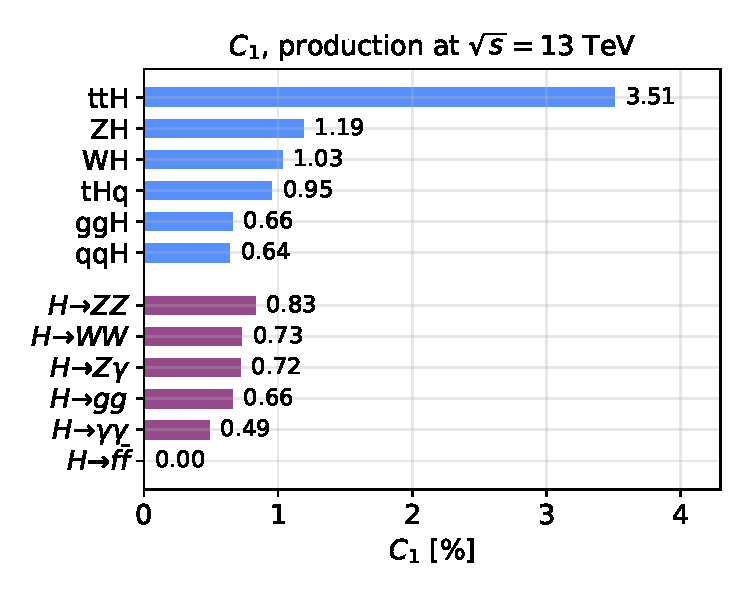
\includegraphics[width=0.49\textwidth]{single_higgs_ch/figures/c1_by_channel.pdf}
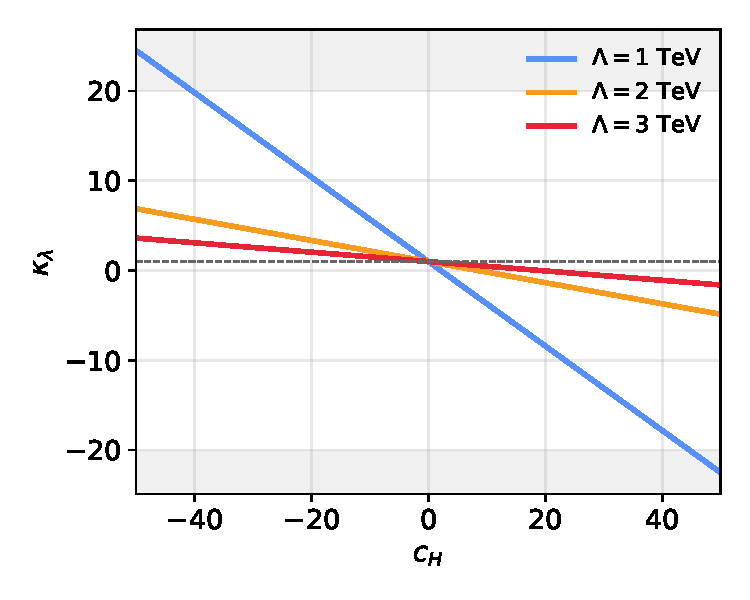
\includegraphics[width=0.49\textwidth]{single_higgs_ch/figures/kappa_lambda_vs_cH.pdf}
\caption{Left: inclusive $C_1$ coefficients of the single-Higgs production modes at
$\sqrt{s}=13$~TeV and of the Higgs
decays~\cite{Degrassi:2016wml,Maltoni:2017ims,Degrassi:2019yix}. Right: the naive
translation of Eq.~\eqref{eq:naivetranslation} from $c_\PH$ to $\kappa_\lambda$ for
three values of the EFT scale; the grey bands mark $|\kappa_\lambda|>20$. Both as in
the model of Ref.~\cite{multihmodels}.}
\label{fig:c1values}
\end{figure}

The translation has three limitations. $C_1$ is computed with only the trilinear

coupling rescaled; a consistent SMEFT calculation at the same order has further
one-loop contributions from the other operators, and operator mixing. An
$\mathcal{O}(\Lambda^{-2})$ coefficient enters a one-loop correction, so the result
is the leading self-coupling effect rather than a complete order in the EFT
expansion. Eq.~\eqref{eq:c1master} is quoted as valid for
$|\kappa_\lambda|<20$~\cite{Maltoni:2017ims}, $85\%$ of the $c_\PH$ range at
$\Lambda=1$~TeV, and the larger $|c_\PH|$ lie outside the region where the
dimension-6 truncation holds (Sec.~\ref{sec:truncation}).

The branching ratios change through the spread of $C_1^i$ across decays,
Eq.~\eqref{eq:brratio} (Fig.~\ref{fig:sh_br}). $\PQb\PAQb$ carries $58\%$ of the
width with $C_1=0$, so the fermionic branching ratios move opposite to the bosonic
ones: over the $c_\PH$ range, $\mathrm{BR}(\PZ\PZ)$ changes by up to $15\%$,
$\mathrm{BR}(\gamma\gamma)$ by $6\%$ and $\mathrm{BR}(\PQb\PAQb)$ by $6\%$ in the
opposite direction. $c_{\PH\mathrm{kin}}$, the coefficient of the Higgs
kinetic term, acts differently. Removing it by a field
redefinition rescales every single-Higgs coupling by the same factor, so that each
partial width scales as
Eq.~\eqref{eq:chkinwidth}
The rescaling cancels between the partial and the total width, and over the
$c_{\PH\mathrm{kin}}$ range of Table~\ref{tab:SMEFTcouplings} the branching ratios
change by less than $1\%$, only through the $c_{\PH\mathrm{kin}}$ term of
Eq.~\eqref{eq:naivetranslation}.

\begin{figure}[htp]
\centering
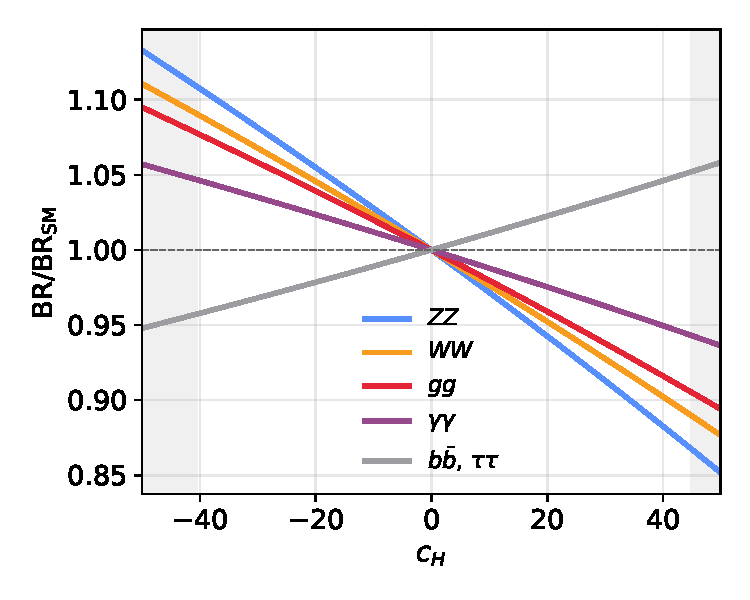
\includegraphics[width=0.49\textwidth]{single_higgs_ch/figures/br_ratio_vs_cH.pdf}
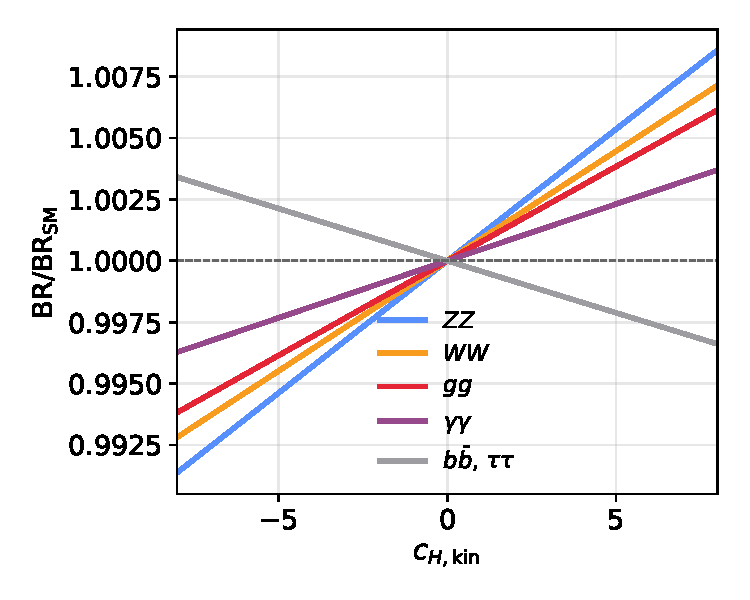
\includegraphics[width=0.49\textwidth]{single_higgs_ch/figures/br_ratio_vs_cHkin.pdf}
\caption{Higgs branching ratios normalized to their SM values as a function of
$c_\PH$ (left) and of $c_{\PH\mathrm{kin}}$ (right), at $\Lambda=1$~TeV;
$\tau\tau$ is identical to $\PQb\PAQb$. The grey bands on the left mark
$|\kappa_\lambda|>20$.}
\label{fig:sh_br}
\end{figure}


\begin{figure}[htp]
\centering
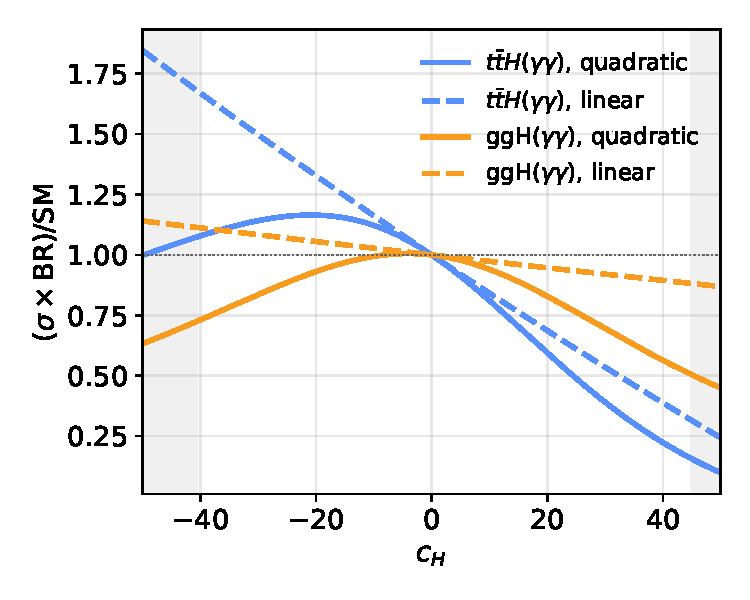
\includegraphics[width=0.52\textwidth]{single_higgs_ch/figures/sigma_times_br_vs_cH.pdf}
\caption{\textcolor{red}{[AUTHORS ONLY]} $\sigma\times\mathrm{BR}$ normalized to the SM for $\ttH(\gamma\gamma)$ and
$\ggH(\gamma\gamma)$, with the scaling of Eq.~\eqref{eq:c1master} in full (solid) and
truncated at first order in $\kappa_\lambda-1$ (dashed), as a function of $c_\PH$ at
$\sqrt{s}=13$~TeV and $\Lambda=1$~TeV, from the model of Ref.~\cite{multihmodels}; the
grey bands mark $|\kappa_\lambda|>20$.}
\label{fig:sh_rates}
\end{figure}

\paragraph{Dependence on the collision energy.}
\label{sec:singleh_ecm}

The decay coefficients $C_1^{i}$ are properties of the Higgs boson, so
Eq.~\eqref{eq:brratio} and the bound of Eq.~\eqref{eq:chkinbound} hold at every
energy. The production coefficients are tabulated at $7$, $8$, $13$ and
$14$~TeV~\cite{Degrassi:2016wml} and decrease slowly with energy ($3.87$, $3.78$,
$3.51$ and $3.47\%$ for \ttH). The model of Ref.~\cite{multihmodels} uses the
$13$~TeV values at $13.6$~TeV as well; the whole $13\to14$~TeV change is at most
$1.1\%$ relative. At $100$~TeV the production coefficients are not computed; their
evaluation requires the phase-space integration and parton-density convolution of
Refs.~\cite{Degrassi:2016wml,Maltoni:2017ims} redone at that energy.

At FCC-ee, at $\sqrt{s}=240$ and $365$~GeV~\cite{FCC:2018evy} and below the
$e^+e^-\to\PZ\HH$ threshold, $c_\PH$ is constrained only through the loop corrections
to $e^+e^-\to\PZ\PH$ and $\PGn\PAGn\PH$, the two energies separating the
self-coupling from the other Higgs couplings~\cite{DiVita:2017vrr}. The expected
precision is of order $30\%$ on $\kappa_\lambda$ from FCC-ee alone, better in
combination with the HL-LHC~\cite{Maura:2025fcc}, and its combination with \HH
requires both expressed in the same Wilson coefficients. Per unit $c_\PH$,
$e^+e^-\to\PZ\PH$ at $240$~GeV ($C_1\simeq1.5\%$~\cite{McCullough:2013ria}) is less
sensitive than \ttH (Fig.~\ref{fig:sh_fccee}); its weight comes from the precision of
the cross-section measurement. \textcolor{red}{\textbf{Oscar, Jon would you keep FCCee in
this paper? It would enrich discussion with not much work, but it is slightly off
topic.}}

\begin{figure}[htp]
\centering
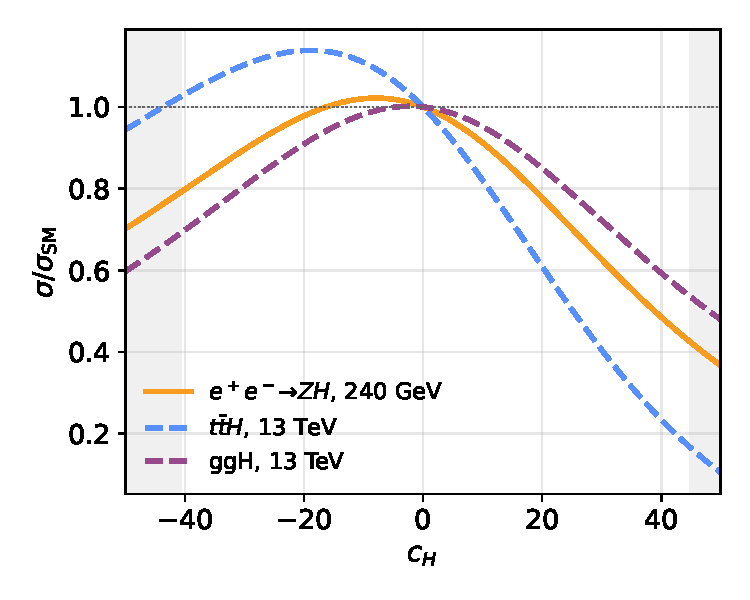
\includegraphics[width=0.62\textwidth]{single_higgs_ch/figures/fccee_vs_lhc_vs_cH.pdf}
\caption{Production cross sections normalized to their SM values as a function of
$c_\PH$ at $\Lambda=1$~TeV: $e^+e^-\to\PZ\PH$ at $\sqrt{s}=240$~GeV (solid), and \ttH
and \ggH at $\sqrt{s}=13$~TeV (dashed). The grey bands mark $|\kappa_\lambda|>20$.
\textcolor{red}{The $365$~GeV curves, and the $WW$-fusion channel, require $C_1$
values that are not yet filled in.} \textcolor{red}{\textbf{Jon, would you be able
to do?}}}
\label{fig:sh_fccee}
\end{figure}

At $\Lambda=1$~TeV a $5\%$ change of the inclusive \ttH rate requires $c_\PH\simeq3$,
small against the present experimental uncertainty on the \ttH cross section. The
term makes the parameterization consistent: $c_\PH$ enters both sides of the
combination, and its correlation with the coefficients \ttH constrains, notably
$c_{\PQt\PH}$, is propagated. With HL-LHC precision on \ttH and the differential
$C_1$ of Ref.~\cite{Maltoni:2017ims} the term becomes a constraint.

\textcolor{red}{TODO: cross-check the production curves against an explicit
\texttt{MG5\_aMC@NLO} evaluation and quote the residual scale and
$m_\PQt$-scheme uncertainty on $C_1$; extend to the differential level in
$p_{\mathrm{T}}^{\PH}$, where $C_1$ is enhanced at threshold; and decide whether
to commission a $100$~TeV computation of $C_1$ to match the reach of
Sec.~\ref{sec:extraction}.} \textcolor{red}{\textbf{Jon, would you be able to do?}}

\section{\textcolor{red}{[AUTHORS ONLY]} The basis for the linear truncation}
\label{sec:appendix_linear}
\label{sec:basis_linear}

\textcolor{red}{\textbf{MATHEUS:} this section records a basis that \emph{did not
work}, and is kept for us rather than for publication. The ten-point basis for the
truncated parametrisation is withdrawn: its basis points are themselves truncated
objects, and after the 4b selections four of the ten have a negative yield in the fully
merged region and one is negative everywhere while its inclusive cross section stays
positive. The ten points and `basis\_linear.txt` have been removed from multih-models
and `model\_linear` now uses the forty points with the formula truncated at evaluation
--- see `HANDOFF\_linear\_truncation\_via\_40point\_basis.md`. The linear-only 4b CSVs
built on the old ten labels need rebuilding or retiring.}

An analysis may choose to keep the effective-field-theory expansion only to the
interference term. That is a different parameterization --- ten monomials
rather than forty --- and it is solved on its own basis, given in
Table~\ref{tab:smeft_basis_linear}. The saving is ten simulated samples instead of forty.

Two points about using it. The coefficients are
\emph{not} obtained by fitting the ten-term system. They are the coefficients of
the full forty-term solve, restricted to the ten linear monomials, which are
$A_0$ to $A_4$ and $A_{15}$ to $A_{19}$ --- not the first ten. Truncating the
formula this way does reproduce samples generated with the same truncation;
fitting the truncated system directly does not. And the ten points of
Table~\ref{tab:smeft_basis_linear} are the basis of the truncated
parameterization, so they are to be used with the truncated formula and not
mixed with the forty points of Table~\ref{tab:smeft_basis_9d}.

The problem is easier than the quadratic one, and for a structural reason: every
monomial here involves at most \emph{one} coupling, where the quadratic
parameterization is two-local. The natural basis would then be the Standard
Model plus one single-coefficient point per coupling. That is not constructible
from the available grid, which has single-coefficient samples only for the four
four-fermion coefficients, so the same two-coupling restriction is applied; the
resulting basis is nevertheless well conditioned, $8.50$ against $32.7$ for the
forty-point one.

One pathology is specific to the truncation and has to be stated. The search
returns, if nothing prevents it, points whose \emph{truncated} total cross
section is negative --- two of ten, at $-598$ and $-39$~fb. Requiring a positive
total removes them, at a cost of $0.4\%$ in the score, which is inside the
seed-to-seed spread. The constraint acts on the total only, and the differential
prediction is not so easily repaired: six of the ten points have negative bins,
between $8$ and $29$ of the $40$, and four of them predict a negative yield
above $1$~TeV. Whether that matters is a question about the analysis rather than
about the basis, and it is taken up in
Sec.~\ref{sec:validation_realistic}.

% generated by scripts/make_basis_table.py in the basis-optimization toolkit; do not edit by hand
\begin{table}[htbp]
\centering\scriptsize
\begin{tabular}{l p{0.38\textwidth} r}
\hline
Point & Non-zero coefficients & $\sigma$ [fb] \\
\hline
BP 01 & SM (all zero) & $31.01$ \\
BP 02 & $c_{\PQt G} = 1$,\; $c_{Q\PQt}^{(1)} = -20$ & $7.238$ \\
BP 03 & $c_{\PQt G} = 1$,\; $c_{Q\PQt}^{(1)} = 20$ & $9.377$ \\
BP 04 & $c_{Q\PQt}^{(8)} = -20$,\; $c_{QQ}^{(8)} = 20$ & $34.44$ \\
BP 05 & $c_{Q\PQt}^{(8)} = -20$,\; $c_{QQ\PQt\PQt} = 20$ & $34.54$ \\
BP 06 & $c_{QQ\PQt\PQt} = 20$,\; $c_{QQ}^{(8)} = 20$ & $31.16$ \\
BP 07 & $c_{\PH\mathrm{kin}} = -8$,\; $c_{\PH G} = -0.1$ & $178.4$ \\
BP 08 & $c_{\PQt\PH} = -10$,\; $c_{\PH G} = -0.0567$ & $4.938$ \\
BP 09 & $c_{\PH} = 50$,\; $c_{\PH G} = -0.0856$ & $742.3$ \\
BP 10 & $c_{\PH\mathrm{kin}} = 8$,\; $c_{\PH G} = -0.1$ & $68.6$ \\
\hline
\end{tabular}
\caption{The ten points of the basis for the linear truncation. Only the coefficients that differ from zero are listed; all others vanish. Every point other than the SM activates exactly two coefficients. Cross sections are evaluated from the inclusive coefficients of the reweighting fit, restricted to the ten linear monomials.}
\label{tab:smeft_basis_linear}
\end{table}


Fig.~\ref{fig:basis_shapes_linear} shows the \mHH distribution of each of the
ten points, normalized to its own yield, in the same format as
Fig.~\ref{fig:basis_shapes}. The contrast with the forty-point basis is the
point of showing it. There, the points fall into four kinematic regimes and the
fraction of the yield above $1$~TeV spans $0.8\%$ to $18\%$. Here all ten
classify as SM-like, and the same fraction runs from $3.3\%$ down to
$-56\%$: the truncated prediction has no access to the hard-tail regime, and
where the interference exceeds the SM term it goes negative rather
than small. This is a property of the truncation and not of the basis --- the
points themselves reach $c_\PH=50$ --- and it is the reason the usability
question of Sec.~\ref{sec:validation_realistic} is posed in terms of the
observable being fitted.

\begin{figure}[htbp]
    \centering
    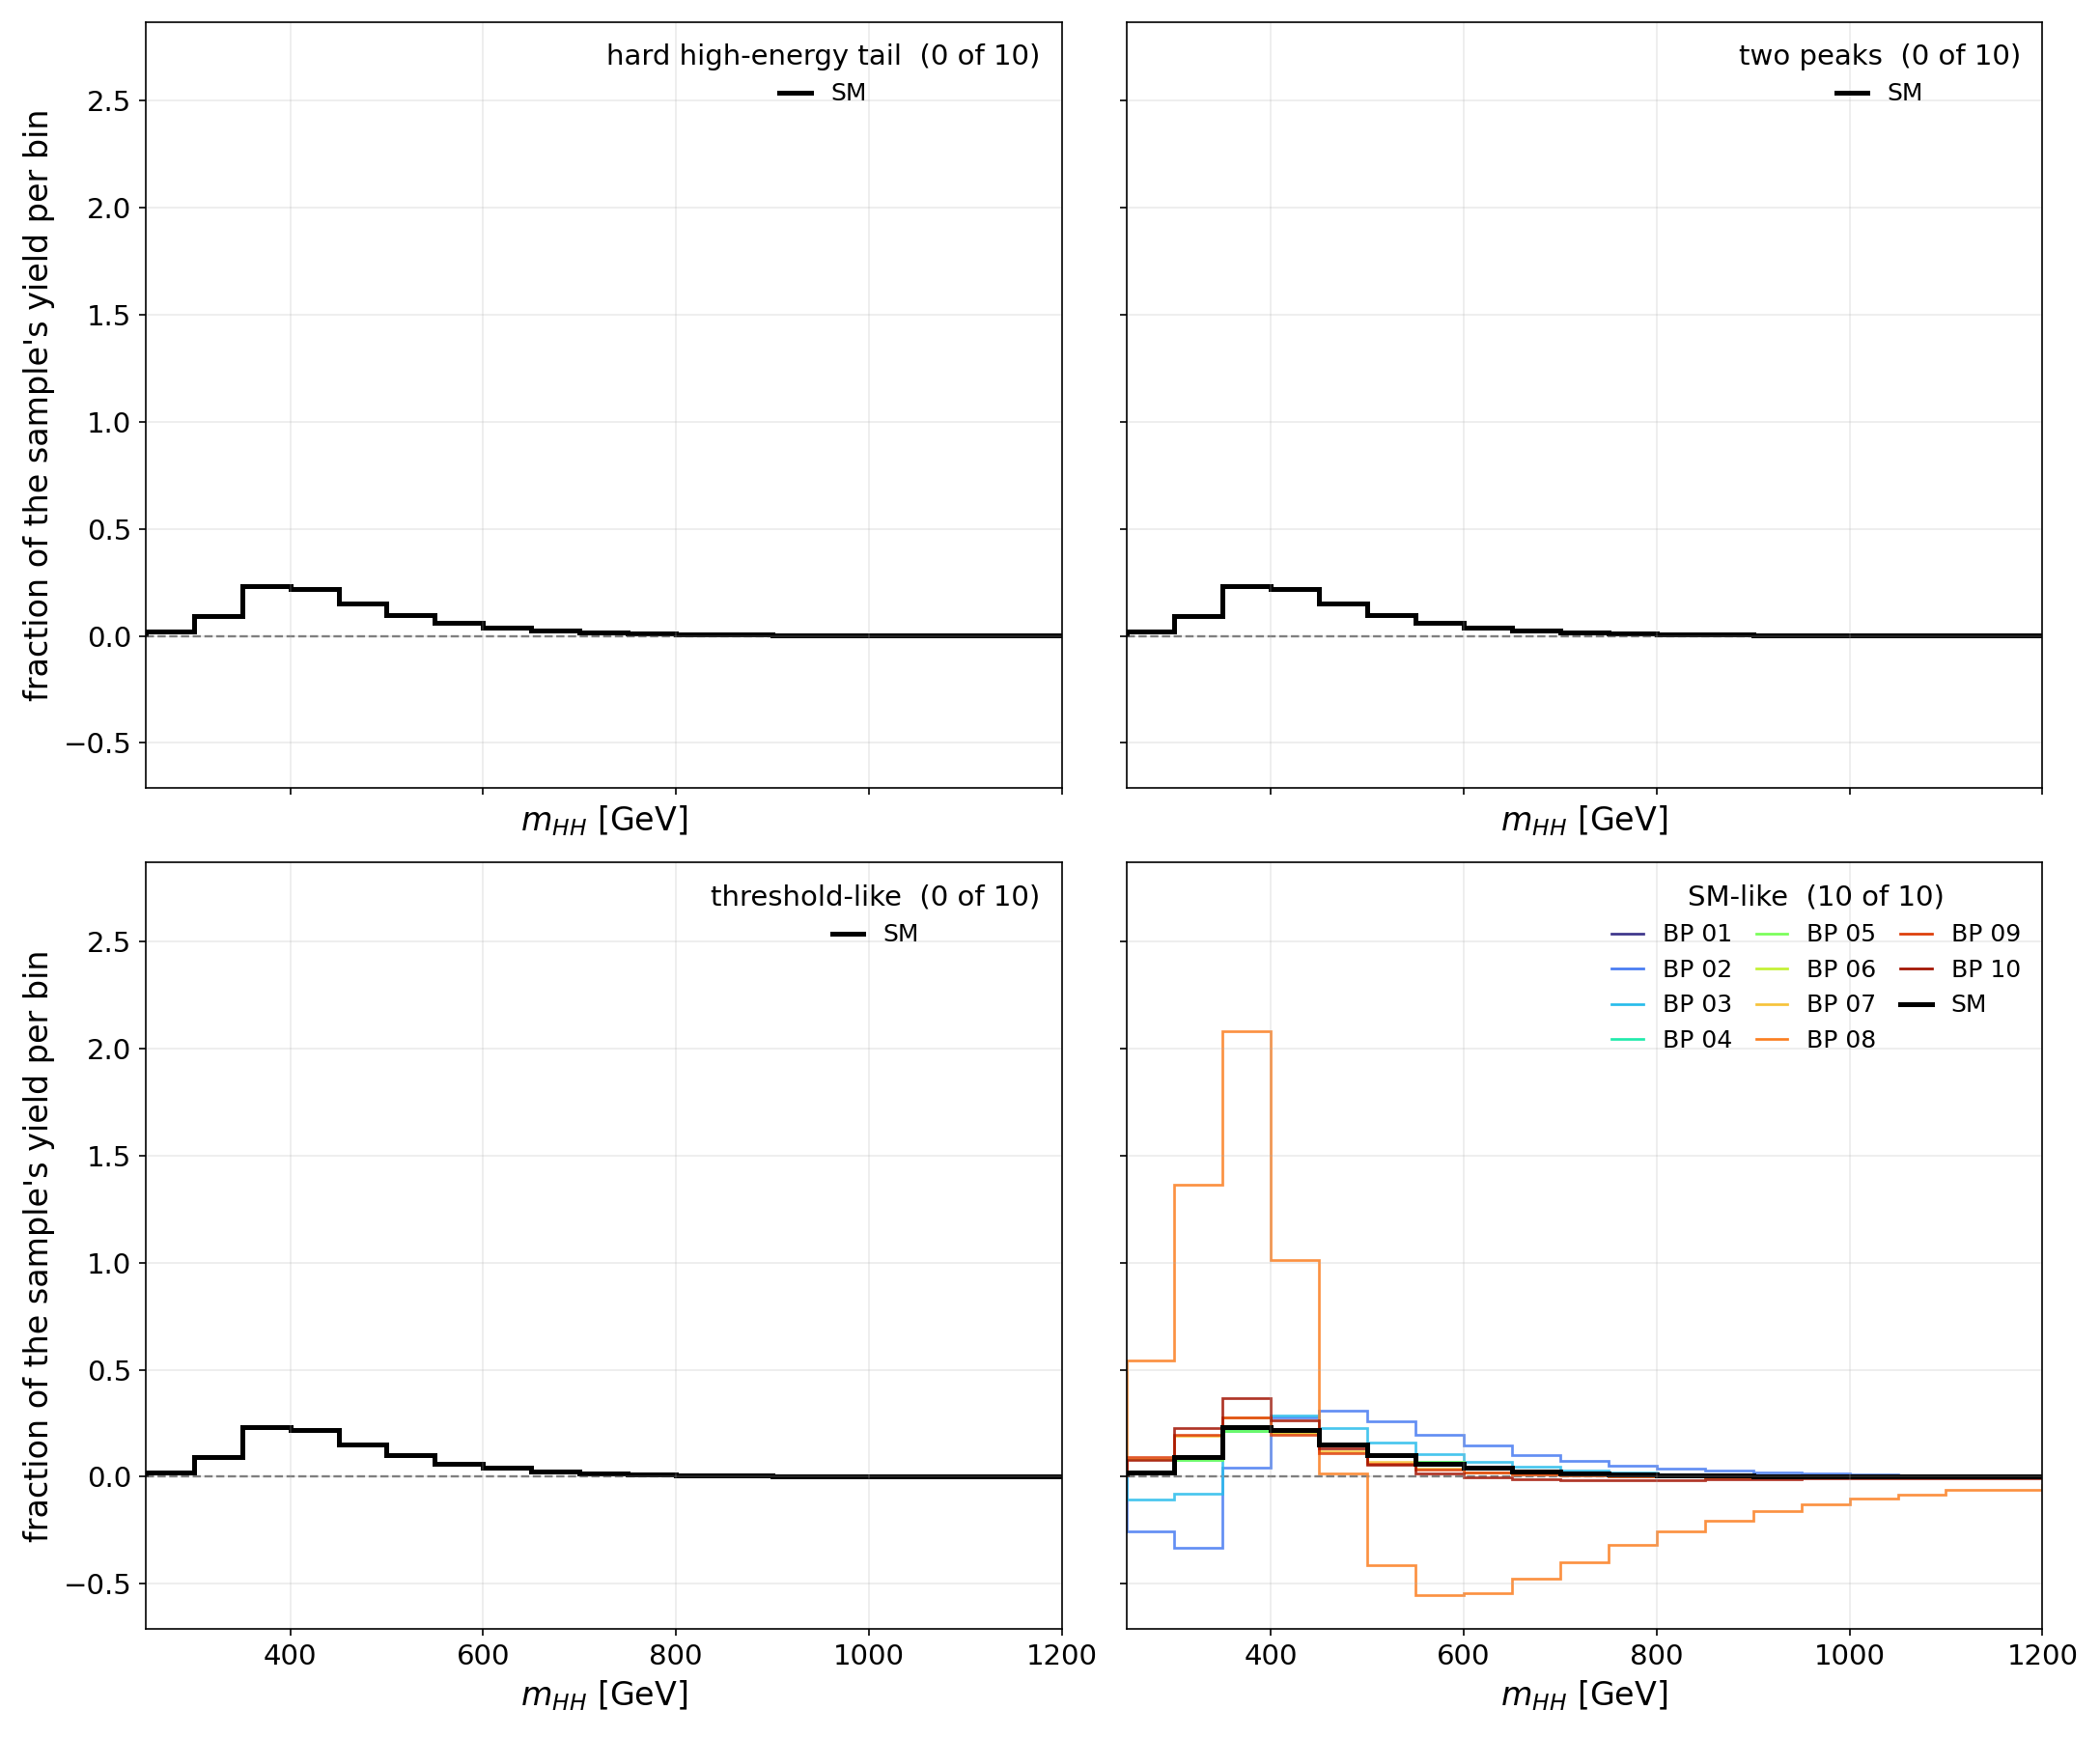
\includegraphics[width=0.70\textwidth]
        {figures/basis_optimization/basis_shapes_linear.png}
    \caption{Normalized \mHH distribution of each of the ten points of the
    linear basis, with the SM drawn in black. Each histogram is
    divided by its own integral. Bins in which the truncated prediction is
    negative are drawn as such; the dashed line marks zero.}
    \label{fig:basis_shapes_linear}
\end{figure}

Fig.~\ref{fig:basis_convergence_linear} shows the search, every seed of the
sweep. It converges far more readily than the quadratic one: the final score
spreads by a factor $1.09$ over the seeds, against $1.34$ for the forty-point
basis, and a seed accepts a median of $13$ exchanges against $91$. Both follow
from the candidate set being small --- the positive-total requirement and the
two-coupling restriction leave $1135$ of the $4376$ pool samples --- and from
the ten-term system being easier to span. The practical consequence is that the
sweep matters less here than it does for the quadratic basis, where it is part
of the procedure.

\begin{figure}[htbp]
    \centering
    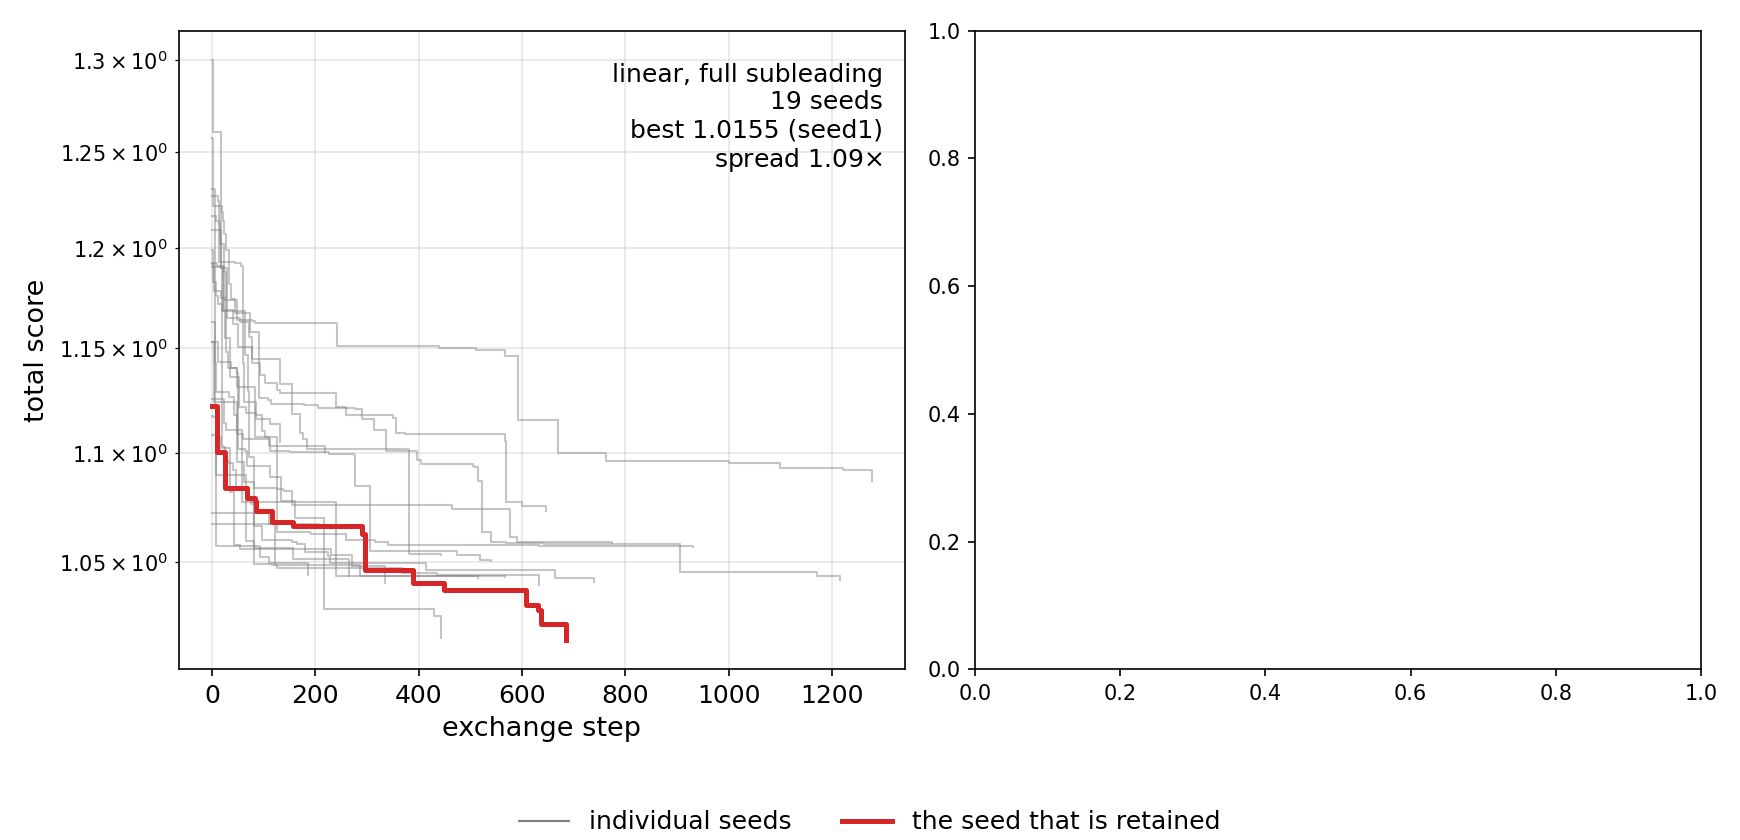
\includegraphics[width=0.60\textwidth]
        {figures/basis_optimization/basis_convergence_linear.png}
    \caption{Total score against exchange step for every seed of the linear
    basis search; the retained seed is highlighted.}
    \label{fig:basis_convergence_linear}
\end{figure}

\subsection{The linear truncation after a selection}
\label{sec:appendix_linear_selection}
The ten points of Sec.~\ref{sec:basis_linear} exist so that an analysis
truncating at the interference term can do so with ten samples instead of
forty. Whether that is a saving or a false economy is a question only this
section can answer, because it depends on what is being fitted and on which
part of phase space is kept.

Without any selection the truncated templates are already difficult: six of the
ten basis points have between $8$ and $29$ negative bins of $40$, and four
predict a negative yield above $1$~TeV, even though the positivity constraint
imposed during the search keeps every inclusive total positive. Where the
interference term exceeds the SM one the truncated cross section
goes negative rather than small. A fit to a rate need not notice; a fit to a
shape cannot use a template that is negative in most of its bins.

After a selection the bin-level problem does not go away,
it only moves: in the binning the datacard actually uses, six of the ten
templates still have negative bins, between two and twelve of twenty-three. Beyond that, the problem stops being about individual bins at all. Of the ten points, four have a
negative yield in the merged selection, and one --- the
point at $c_{\PQt\PH}=-10$, $c_{\PH G}=-0.0567$ --- is negative in every region
while its truncated inclusive cross section is positive. That is not a template
with awkward bins: its integral is negative, so it can enter a fit neither as a
shape nor as a rate.

The reason is that the positivity constraint acts on the inclusive total, and
inclusive positivity does not survive a selection. A selection reweights the
bins, and one that favours the high-mass tail concentrates exactly the region
where the truncated prediction is most negative. A constraint that would help
has to impose positivity after the analysis's own selection, which a basis
search cannot do in advance because it does not know the selection.

The conclusion is that the ten-point basis is not usable with these selections,
and the question is not whether a shape fit can use the templates but whether a
usable linear basis exists for a given selection at all. Two routes remain. An
analysis restricting its coupling ranges may not meet the problem, since every
negative point lies far from the SM. Otherwise the forty-point
basis with the formula truncated at evaluation time gives a linear prediction
with no negative templates; it is a different object and costs forty samples
rather than ten, and the two are not interchangeable.

\clearpage
\subsection{\textcolor{red}{[AUTHORS ONLY]} The dimension-6 validity criterion, per operator and per bin}
\label{sec:appendix_trunc_validity}

\textcolor{red}{For the authors. The criterion itself is not ours --- restricting to where
the interference dominates the dimension-6 square is the standard prescription, and the
threshold is a convention with no first-principles answer~\cite{Contino:2016jqw,Brivio:2017vri}. What is
ours is the evaluation below: the same criterion applied to the nine coefficients of this
report, differentially in \mHH rather than inclusively, from the fitted
$A$-coefficients. It is kept here rather than in the main text because it supports a
statement the literature already makes, and because the numbers depend on a threshold we
chose.}

\begin{table}[htbp]
\centering
\begin{tabular}{l|cccc}
\hline
operator & inclusive & $\mHH \in [400,410]$~GeV & $\mHH \in [1000,1050]$~GeV & $\mHH \in [1400,1500]$~GeV \\
\hline
$c_{\PH}$              & $5.6$ & $9$ & $21.5$ & $28.4$ \\
$c_{\PH\mathrm{kin}}$  & $7.8$ & $13.9$ & $3.02$ & $1.63$ \\
$c_{\PQt\PH}$          & $7.21$ & $13.4$ & $2.25$ & $1.27$ \\
$c_{\PH G}$            & $0.0263$ & $0.0754$ & $0.0092$ & $0.00591$ \\
\hline
\end{tabular}
\caption{\textcolor{red}{[AUTHORS ONLY]} Coupling value $|c|\simeq|A^j_{\text{lin}}/A^j_{\text{quad}}|$ at which the
dimension-6 squared contribution equals the dimension-6 interference, for the four
leading operators, inclusively and in three \mHH bins, at $\sqrt{s}=13.6$~TeV.
$A^j_{\text{quad}}$ is the diagonal entry of the leading quadratic block. The quantity
is defined only for operators with a genuine square.}
\label{tab:trunc_validity}
\end{table}

\clearpage
\section{Details of the basis search}
\label{sec:appendix_basis_search}

The search is that of Ref.~\cite{HH_nonggf_R5}; this appendix gives the five
implementation changes summarized in Sec.~\ref{sec:basis_refinements}, the arguments for
restricting the basis to the planes, and the changes that were tried and did not improve
the result.

\subsection{Why the basis is restricted to the planes}
\label{sec:appendix_basis_planes}

The result is in Sec.~\ref{sec:basis_planes}; the arguments for it are collected here.

The sample grids of Sec.~\ref{sec:grids} are not an unstructured cloud: most of
their points lie in one of the $\binom{9}{2}$ planes in which a single pair of
Wilson coefficients is varied with the rest held at their SM values.
We exploit that structure and require the basis points to be drawn from those
planes, allowing a small number of exceptions.

The restriction is not an approximation. No monomial of
Eq.~\eqref{eq:smeftpara_reorg} involves more than two distinct coefficients: the
$40$ terms are the SM term, the linear terms, the pairwise-quadratic
combinations of the four leading coefficients, and the products of one leading
with one subleading coefficient. The parameterisation is in this sense
\emph{two-local}, and a set of points each of which activates at most two
coefficients is therefore not structurally degenerate.

Two considerations motivate the choice. The first is numerical. Bases selected
from the planes are consistently better conditioned than bases selected from the
whole pool --- condition number $21$ against $33$ for the $20$-point 5D basis,
and $26$ against $40$ for the $40$-point 9D one --- because points that activate
many coefficients at once populate the monomials less distinctly and bring the
basis closer to degeneracy. The second is interpretational. Every basis point
then isolates one coefficient pair, so each template can be attributed to a
specific pair of operators, and the basis maps directly onto the
two-dimensional scans in which the results of such analyses are presented.

The restriction was initially applied with a budget of a few exceptions, on the
expectation that it would not be free: a basis drawn only from the planes might
be more accurate on plane targets and less accurate on the rest, and the points
that activate many coefficients make up the majority of the sample set. That
expectation turned out to be wrong, and the budget is not used.

Only the \emph{membership} of the basis is restricted. The
validation targets against which every candidate basis is scored are never restricted:
the loss asks a candidate to predict every other sample in the grid, and at $13.6$~TeV
$2792$ of the $4376$ samples --- about two thirds --- activate more than two
coefficients. The basis is therefore always required to describe the full parameter
space, and is selected on its ability to do so; what is structured is only the set of
points it may be built from.

Scoring the twenty converged seeds against on-plane targets alone and against
off-plane targets alone gives rankings with a Spearman correlation of $0.24$: the basis
that is best on the planes ranks sixteenth of twenty off them, while the basis adopted
here is first off the planes and third on them. Off the planes the interpolation error
and the morphing weight norms are both about $1.6$ times larger. A grid of plane scans
alone would therefore determine the coefficients, but would not discriminate between
candidate bases.

The full sweep settles it. Every one of the $40$ points of the recommended
nine-coefficient basis lies in a two-dimensional plane: thirty-nine activate
exactly two coefficients and one is the SM. Its condition number is
$32.7$ and its total score $0.609$, against $18.4$ and $0.359$ for the
twenty-point basis and $12.7$ and $0.305$ for the fifteen-point one; the score is
not comparable between parameterizations of different size, since it is dominated
by terms that grow with the number of monomials. Allowing two points off the
planes was tested on the same footing, as a separate twenty-seed sweep: it gives
a slightly worse score ($0.624$) and a measurably worse closure against the
generated samples ($3.5\%$ against $3.0\%$ in median relative shape residual,
Sec.~\ref{sec:validation_mm}), at a slightly better condition number ($26.6$).
The restriction therefore costs nothing in accuracy, and every basis point lies in a
plane the results are presented in.

\subsection{Refinements to the search, and what did not improve it}
\label{sec:appendix_basis_refinements}
\label{sec:basis_difficulty}

Five changes with respect to the search of Ref.~\cite{HH_nonggf_R5}:

\begin{itemize}
  \item \emph{Degeneracy of randomly drawn starting configurations.} Ref.~\cite{HH_nonggf_R5} initializes each seed from the best of several starting configurations, one of which is a set of purely random selections. In nine dimensions a randomly drawn configuration is almost always singular, for a counting reason rather than through bad luck. Of the $40$ monomials of Eq.~\eqref{eq:smeftpara_reorg}, $20$ vanish unless one of the four four-fermion coefficients is non-zero, while only $45\%$ of the generated samples have one; a uniform draw of $40$ points therefore contains about $18$ such samples where $20$ are needed, and we find that $85\%$ of random draws give a rank-deficient interpolation matrix. The random starting configurations are accordingly redrawn until the matrix has full rank, which restores all of them to use. The effect is absent at the dimensionality of Ref.~\cite{HH_nonggf_R5}, where the corresponding fraction is negligible, and it grows with the number of coefficients that enter the parameterization only through products.
  \item \emph{Rank in the well-conditioned starting configuration.} The second starting configuration of Ref.~\cite{HH_nonggf_R5} is the one that favours well-conditioned interpolation matrices, built greedily by adding at each step the sample that most increases the pseudo-determinant. Ranking candidates by the pseudo-determinant alone is not safe when the matrix is still rank deficient: discarding a vanishing singular value increases the product over the surviving ones, so a selection that keeps the matrix degenerate can score higher than one that does not. We therefore rank candidates first by the rank of the matrix and only then by the pseudo-determinant. The two orderings agree whenever the candidate samples are unstructured, which is why this does not affect the bases of Ref.~\cite{HH_nonggf_R5}; they differ when the candidates are restricted, as they are by the two-dimensional plane requirement of Sec.~\ref{sec:basis_planes}, where the unmodified ranking returns a basis one short of full rank even when every candidate is examined.
  \item \emph{Validation targets.} Ref.~\cite{HH_nonggf_R5} evaluates every candidate basis against every sample of the optimization set. Preserving that at the sample sizes of this report is a question of implementation rather than of method: evaluating the score for all targets at once, rather than one target at a time, reduces its cost by a factor of about five and keeps the full optimization set affordable at every exchange step. No subsampling of the targets is therefore used, and the scores quoted here are computed on the complete set.
  \item \emph{Number of basis points.} The bases of Ref.~\cite{HH_nonggf_R5} are exactly determined: as many samples as coupling structures, so that the interpolation matrix is square and inverted exactly. We retain that as the default and allow, as an option, more samples than structures. The interpolation weights are then the minimum-norm least-squares solution, which distributes the weight of a target over more samples and so averages down the statistical uncertainty each of them carries. This is the unweighted counterpart of the statistically aware extension of Ref.~\cite{HHMatrix_R5}: it spreads the weights but treats every sample as equally reliable, whereas Ref.~\cite{HHMatrix_R5} weights them by their covariance. Recovering the full procedure requires per-bin uncertainties to be propagated with the samples. The bases reported here are all exactly determined.
  \item \emph{Recording the convergence.} Ref.~\cite{HH_nonggf_R5} notes in its appendix that the step-by-step trace of the published runs was written only to the standard output of the batch jobs and did not survive with the results, so that no convergence information could be reported. The optimization used here writes the accepted exchanges and the value of every term of the score to a file as the search proceeds, so a run that is interrupted still leaves its convergence behind.
\end{itemize}

Figure~\ref{fig:basis_convergence} shows those trajectories for the two ends of the
ladder, every seed of each. Three things follow. The descent is fast and then stops: by
step $50$ a seed has already made $90\%$ of the total improvement it will ever make for
the fifteen-point basis, and $83\%$ for the forty-point one. The seeds do not converge
to a common value, and the spread of their final scores is far larger than the few per
cent of improvement still available after step $200$: they differ not in how far they
descend but in which local optimum they reach, which is also why the starting
configuration does not predict the outcome (the rank correlation between initial and
final score is $+0.08$ and $+0.22$). And a seed cannot be judged early: ranking the
seeds by their score at step $50$ has rank correlation $-0.09$ and $-0.11$ with their
final ranking, and at step $200$, with most of the improvement already banked, still
only $+0.45$ and $-0.06$. Starting many seeds, keeping the best few and letting only
those finish would therefore select close to at random for the nominal basis: the
ordering is settled in the long, nearly flat tail of the trajectory, where little score
is gained but the basis is still being rearranged. Every seed is run to its own
stopping rule.

\begin{figure}[htbp]
    \centering
    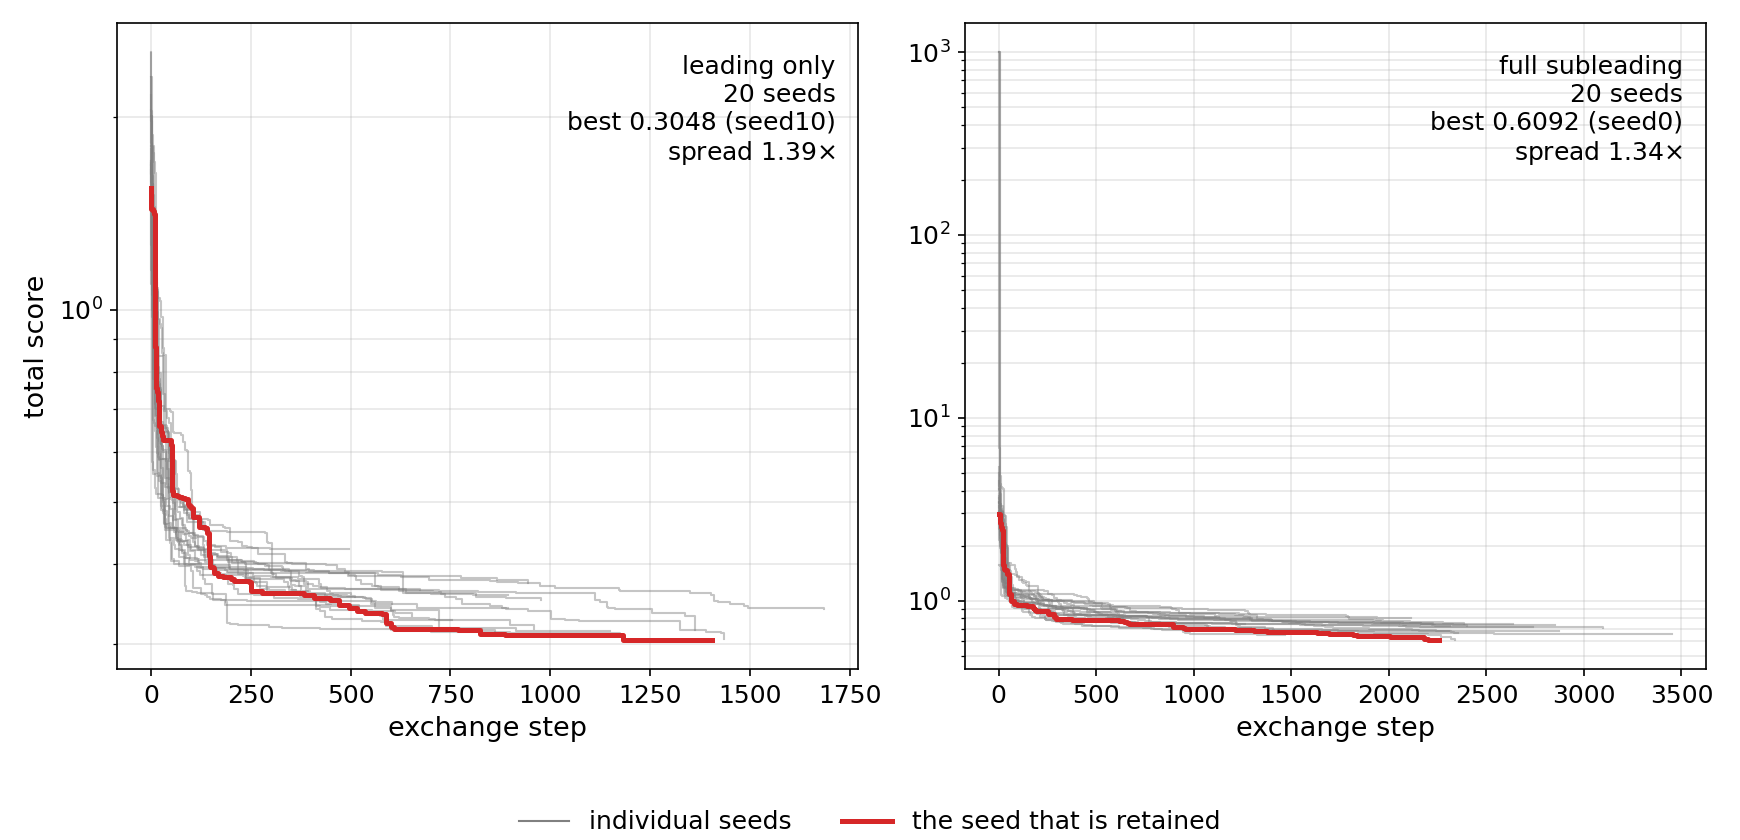
\includegraphics[width=0.92\textwidth]
        {figures/basis_optimization/basis_convergence.png}
    \caption{Total score against exchange step for each of the $20$ seeds of the
    fifteen-point (left) and forty-point (right) optimizations; the seed that is
    retained is highlighted. Each line is a staircase of accepted exchanges, taken from
    the record the search writes as it proceeds. Only accepted exchanges appear as
    steps, so the flat stretches are not idle: each step probes $30$ candidate
    replacements. The score is not comparable between the two panels, being dominated
    by terms that grow with the number of monomials.}
    \label{fig:basis_convergence}
\end{figure}

Each parameterization was optimized with $20$ independent seeds. The searches accept a
median of $47$ exchanges and stop after $300$ consecutive steps without an improvement.
The spread of the final score over seeds is a factor $1.39$, $1.31$ and $1.34$ for the
fifteen-, twenty- and forty-point cases, so one run does not determine the basis and
the sweep is part of the procedure.

Four further changes were tried and did not improve the result:

\begin{itemize}
  \item \emph{Penalizing the norm of the interpolation weights.} The residual of
    the matrix method is dominated by the statistical error of the basis samples
    propagated through those weights, so penalizing their quadratic norm appears
    to address the dominant term directly. It does not: over the seeds of the
    nine-coefficient sweep the norm is weakly \emph{anti}-correlated with the
    delivered residual (Spearman $-0.18$), and selecting on it gives $4.2\%$
    against the $3.5\%$ of the score. The term is used only for the truncated
    parameterizations, where the closure terms vanish identically and the weight
    norms are the only quantity that varies between bases.
  \item \emph{Selecting the seed on the validation rather than on the score.}
    This does improve the median residual, by $24\%$, $3\%$ and $13\%$ for the
    three parameterizations, but it degrades the tail where the two disagree: for
    the nominal basis the $99$th percentile worsens from $0.21$ to $0.24$. The
    score is weighted towards the worst case, so the two criteria answer different
    questions. We retain the score, and quote the validation separately in
    Sec.~\ref{sec:validation}.
  \item \emph{Over-determined bases.} An optimized exactly-determined basis was the
    better of the two at equal cost, and the same statistical gain is obtained more
    effectively by building the basis points from a few samples by reweighting
    (Sec.~\ref{sec:validation_nsamples}).
  \item \emph{Exhausting the neighbourhood before stopping.} The search stops
    after $300$ steps without an improvement rather than after proving that no
    single exchange improves. An exhaustive sweep of the $8520$ single-exchange
    neighbours of a converged basis found four improving moves, the best of them
    $1.5\%$ of the score, and that move left the median residual unchanged.
    The stopping rule is therefore not what limits the result.
\end{itemize}

The basis is optimized at $\sqrt{s}=13.6$~TeV, the main energy of this report. Since the \ggHH kinematics at $13$~TeV are very close to those at $13.6$~TeV, the same basis is applicable there without being re-optimized. \textcolor{red}{PLACEHOLDER: at $100$~TeV the kinematics change substantially, the spectrum extending to much higher \mHH and the relative weight of the diagrams shifting accordingly; we still have to see how much the basis is affected and whether the matrix method, with a basis optimized in this way, is applicable at that energy at all. The ELR coefficients are in any case provided at $100$~TeV.}

The resulting basis for the nominal nine-coefficient parameterization is given in
Table~\ref{tab:smeft_basis_9d}. It is the default of this report; the bases of the
two reduced parameterizations are used only for the comparisons of
Sec.~\ref{sec:validation} and are not reproduced here.

% Generated by scripts/make_basis_table.py in the basis-optimization toolkit
% (--layout sparse). The dense nine-column layout the script can also produce is
% not used: every point activates exactly two coefficients, so seven of the nine
% columns would be zero on every row.
% generated by scripts/make_basis_table.py in the basis-optimization toolkit; do not edit by hand
%\begin{table}[htbp]
%\centering\scriptsize
%\begin{tabular}{l p{0.26\textwidth} r|l p{0.26\textwidth} r}
%\hline
%Point & Non-zero coefficients & $\sigma$ [fb] & Point & Non-zero coefficients & $\sigma$ [fb] \\
%\hline
%BP 01 & SM (all zero) & $31.01$ & BP 21 & $c_{\PH\mathrm{kin}} = -8$,\; $c_{QQ\PQt\PQt} = -20$ & $141.7$ \\
%BP 02 & $c_{\PH G} = -0.0567$,\; $c_{\PQt G} = 1$ & $120.9$ & BP 22 & $c_{\PH} = -27.8$,\; $c_{QQ}^{(8)} = -20$ & $1424$ \\
%BP 03 & $c_{\PH G} = -0.0711$,\; $c_{QQ}^{(8)} = 20$ & $274.7$ & BP 23 & $c_{\PH} = -27.8$,\; $c_{\PH\mathrm{kin}} = -2.67$ & $1264$ \\
%BP 04 & $c_{\PH G} = -0.0856$,\; $c_{Q\PQt}^{(1)} = -20$ & $346.6$ & BP 24 & $c_{u\PH} = 7$,\; $c_{QQ\PQt\PQt} = -10$ & $139.1$ \\
%BP 05 & $c_{\PH G} = -0.1$,\; $c_{Q\PQt}^{(1)} = 10$ & $486.7$ & BP 25 & $c_{\PH\mathrm{kin}} = 8$,\; $c_{u\PH} = -10$ & $210.5$ \\
%BP 06 & $c_{\PH G} = -0.1$,\; $c_{QQ\PQt\PQt} = -10$ & $473.8$ & BP 26 & $c_{\PH\mathrm{kin}} = 8$,\; $c_{QQ\PQt\PQt} = 20$ & $32.18$ \\
%BP 07 & $c_{\PH\mathrm{kin}} = 8$,\; $c_{\PQt G} = 1$ & $47.94$ & BP 27 & $c_{u\PH} = 1.33$,\; $c_{Q\PQt}^{(8)} = -20$ & $47.06$ \\
%BP 08 & $c_{\PH\mathrm{kin}} = 8$,\; $c_{\PH G} = -0.0711$ & $110.7$ & BP 28 & $c_{\PH G} = -0.0711$,\; $c_{Q\PQt}^{(8)} = -20$ & $269.7$ \\
%BP 09 & $c_{u\PH} = -8.11$,\; $c_{\PQt G} = 0.675$ & $48.25$ & BP 29 & $c_{\PH} = -16.7$,\; $c_{\PQt G} = 0.675$ & $521.6$ \\
%BP 10 & $c_{\PH} = -50$,\; $c_{QQ\PQt\PQt} = -20$ & $5050$ & BP 30 & $c_{u\PH} = -10$,\; $c_{Q\PQt}^{(1)} = -20$ & $66.08$ \\
%BP 11 & $c_{u\PH} = 7$,\; $c_{QQ\PQt\PQt} = 10$ & $139.5$ & BP 31 & $c_{\PH} = 38.9$,\; $c_{QQ\PQt\PQt} = -10$ & $3939$ \\
%BP 12 & $c_{u\PH} = -8.11$,\; $c_{\PH G} = -0.0856$ & $177.3$ & BP 32 & $c_{\PH\mathrm{kin}} = 4.44$,\; $c_{QQ\PQt\PQt} = -20$ & $17.95$ \\
%BP 13 & $c_{\PH} = -38.9$,\; $c_{\PH G} = -0.1$ & $1764$ & BP 33 & $c_{\PH} = -38.9$,\; $c_{\PH\mathrm{kin}} = 6.22$ & $3550$ \\
%BP 14 & $c_{\PH} = -27.8$,\; $c_{Q\PQt}^{(1)} = 20$ & $1391$ & BP 34 & $c_{\PQt G} = 1$,\; $c_{QQ}^{(8)} = -20$ & $8.282$ \\
%BP 15 & $c_{u\PH} = -10$,\; $c_{Q\PQt}^{(1)} = 20$ & $56.78$ & BP 35 & $c_{\PQt G} = 1$,\; $c_{QQ}^{(8)} = 20$ & $8.334$ \\
%BP 16 & $c_{u\PH} = -8.11$,\; $c_{Q\PQt}^{(8)} = -20$ & $40.9$ & BP 36 & $c_{\PH\mathrm{kin}} = -8$,\; $c_{QQ}^{(8)} = -20$ & $142.1$ \\
%BP 17 & $c_{\PH\mathrm{kin}} = -8$,\; $c_{Q\PQt}^{(1)} = 10$ & $145.7$ & BP 37 & $c_{\PH\mathrm{kin}} = 6.22$,\; $c_{Q\PQt}^{(8)} = -20$ & $25.65$ \\
%BP 18 & $c_{\PH\mathrm{kin}} = -8$,\; $c_{Q\PQt}^{(1)} = -20$ & $135.3$ & BP 38 & $c_{\PH\mathrm{kin}} = 2.67$,\; $c_{Q\PQt}^{(1)} = 20$ & $18.08$ \\
%BP 19 & $c_{u\PH} = -8.11$,\; $c_{QQ}^{(8)} = 20$ & $38.9$ & BP 39 & $c_{\PH} = -27.8$,\; $c_{u\PH} = 7$ & $1096$ \\
%BP 20 & $c_{\PH} = -16.7$,\; $c_{Q\PQt}^{(8)} = -20$ & $449.6$ & BP 40 & $c_{\PH} = 5.56$,\; $c_{\PH G} = 0.03$ & $104.7$ \\
%\hline
%\end{tabular}
%\caption{The 40 points of the optimized nine-coefficient basis. Cross sections are evaluated from the inclusive coefficients of the reweighting fit, so they are consistent with the parameterization used to morph the templates. Only the coefficients that differ from zero are listed; all others vanish. Every point other than the SM activates exactly two coefficients, so each lies in one of the pairwise planes.}
%\label{tab:smeft_basis_9d}
%\end{table}

\begin{table}[htbp]
  \centering\scriptsize
  \begin{tabular}{l p{0.26\textwidth} r|l p{0.26\textwidth} r}
  \hline
  Point & Non-zero coefficients & $\sigma$ [fb] & Point & Non-zero coefficients & $\sigma$ [fb] \\
  \hline
  BP 01 & SM (all zero) & $31.01$ & BP 21 & $c_{\PH\mathrm{kin}} = -8$,\; $c_{QQ\PQt\PQt} = -20$ & $141.7$ \\
  BP 02 & $c_{\PH G} = -0.0711$,\; $c_{QQ}^{(8)} = 10$ & $274.5$ & BP 22 & $c_{\PH} = -27.8$,\; $c_{\PH\mathrm{kin}} = -8$ & $981.7$ \\
  BP 03 & $c_{\PH G} = -0.0711$,\; $c_{QQ}^{(8)} = -20$ & $274.1$ & BP 23 & $c_{\PH\mathrm{kin}} = 2.67$,\; $c_{QQ\PQt\PQt} = -20$ & $18.95$
  \\ 
  BP 04 & $c_{\PH G} = -0.0856$,\; $c_{Q\PQt}^{(1)} = 20$ & $387.8$ & BP 24 & $c_{\PH} = -38.9$,\; $c_{u\PH} = -4.33$ & $3321$ \\
  BP 05 & $c_{\PH\mathrm{kin}} = -4.44$,\; $c_{\PQt G} = 0.675$ & $49.22$ & BP 25 & $c_{u\PH} = -6.22$,\; $c_{Q\PQt}^{(8)} = 20$ & $22.09$ \\
  BP 06 & $c_{u\PH} = -10$,\; $c_{\PH G} = -0.0711$ & $102.0$ & BP 26 & $c_{u\PH} = -8.11$,\; $c_{QQ\PQt\PQt} = 20$ & $38.73$ \\ 
  BP 07 & $c_{u\PH} = -10$,\; $c_{\PQt G} = 0.675$ & $76.41$ & BP 27 & $c_{\PH} = -16.7$,\; $c_{QQ\PQt\PQt} = -20$ & $448.6$ \\
  BP 08 & $c_{\PH G} = -0.0711$,\; $c_{Q\PQt}^{(8)} = 20$ & $279.0$ & BP 28 & $c_{\PH\mathrm{kin}} = 8$,\; $c_{\PQt G} = 0.675$ & $42.89$ \\
  BP 09 & $c_{\PH G} = -0.0422$,\; $c_{\PQt G} = 1$ & $70.82$ & BP 29 & $c_{\PH G} = -0.0422$,\; $c_{QQ\PQt\PQt} = -20$ & $131.8$ \\
  BP 10 & $c_{\PH} = -16.7$,\; $c_{\PQt G} = 1$ & $557.0$ & BP 30 & $c_{\PH\mathrm{kin}} = -8$,\; $c_{QQ\PQt\PQt} = 20$ & $142.7$ \\
  BP 11 & $c_{\PH\mathrm{kin}} = 0.889$,\; $c_{u\PH} = -8.11$ & $46.90$ & BP 31 & $c_{\PH} = 16.7$,\; $c_{Q\PQt}^{(1)} = 20$ & $890.3$ \\
  BP 12 & $c_{\PH\mathrm{kin}} = 6.22$,\; $c_{\PH G} = -0.1$ & $285.5$ & BP 32 & $c_{\PH\mathrm{kin}} = 8$,\; $c_{QQ}^{(8)} = 10$ & $32.36$ \\
  BP 13 & $c_{u\PH} = -8.11$,\; $c_{QQ}^{(8)} = -20$ & $39.10$ & BP 33 & $c_{\PH} = -27.8$,\; $c_{u\PH} = 3.22$ & $1259$ \\ 
  BP 14 & $c_{\PH} = -27.8$,\; $c_{\PH G} = -0.0711$ & $835.5$ & BP 34 & $c_{\PH\mathrm{kin}} = -8$,\; $c_{Q\PQt}^{(8)} = 20$ & $138.6$ \\
  BP 15 & $c_{\PH\mathrm{kin}} = -8$,\; $c_{u\PH} = -6.22$ & $43.67$ & BP 35 & $c_{\PH} = 50$,\; $c_{u\PH} = -4.33$ & $5813$ \\
  BP 16 & $c_{u\PH} = 7$,\; $c_{Q\PQt}^{(8)} = -20$ & $144.0$ & BP 36 & $c_{\PH} = -50$,\; $c_{Q\PQt}^{(8)} = -20$ & $5046$ \\
  BP 17 & $c_{\PH} = -5.56$,\; $c_{Q\PQt}^{(1)} = 20$ & $24.97$ & BP 37 & $c_{u\PH} = 7$,\; $c_{Q\PQt}^{(8)} = 20$ & $134.6$ \\
  BP 18 & $c_{\PH\mathrm{kin}} = 8$,\; $c_{Q\PQt}^{(1)} = 20$ & $27.59$ & BP 38 & $c_{u\PH} = -10$,\; $c_{Q\PQt}^{(1)} = -20$ & $66.08$ \\
  BP 19 & $c_{u\PH} = 1.33$,\; $c_{QQ}^{(8)} = -20$ & $43.36$ & BP 39 & $c_{\PH\mathrm{kin}} = 8$,\; $c_{QQ}^{(8)} = -10$ & $32.44$ \\
  BP 20 & $c_{\PH} = 16.7$,\; $c_{QQ}^{(8)} = -20$ & $869.2$ & BP 40 & $c_{\PH\mathrm{kin}} = 6.22$,\; $c_{\PH G} = 0.03$ & $80.39$ \\
  \hline
  \end{tabular}
  \caption{The 40 points of the optimized nine-coefficient basis. Cross sections are evaluated by summing over the differential $A$-coefficients. Only the coefficients that differ from zero are listed, all others vanish. Every point other than the SM activates exactly two coefficients, so each lies in one of the pairwise planes.}
  \label{tab:smeft_basis_9d}
  \end{table}
  



One property of that basis indicates where additional simulation would reduce the
interpolation uncertainty most. The SM point is present in
every candidate basis by construction, and it carries $29.9\%$ of the propagated
interpolation variance of Eq.~\eqref{eq:sigmainterp} on its own, against $9\%$ for the
twenty least important points together. The reason is algebraic rather than kinematic.
At $\mathbf{c}=0$ every monomial of $\varphi$ vanishes except the constant, so the
SM row of the design matrix is the unit vector that alone determines
$A^j_0$; every prediction contains $A^j_0$, so the weight vector of every target has a
large SM component wherever that target sits. Its mean $|w_i|$ is $0.750$,
against a median of $0.074$ over the other thirty-nine points. It is not that the
SM is kinematically central --- by shape distance to the generated set it
ranks only $28$th of the forty.

The consequence is that quadrupling the statistics of that one sample would reduce the
total propagated uncertainty by about $12\%$, which no other single sample approaches,
and it would do so for every target rather than for nearby ones only. It cannot be
arranged away by choosing a different basis, since the effect follows from
$\mathbf{c}=0$ and not from the selection of the other points. This applies when the
basis templates are generated; where they are instead built by reweighting, as in
Sec.~\ref{sec:validation_nsamples}, the statistics of the basis samples largely cease
to matter and the recommendation is superseded.
